% =====================================================================
%  Anatomía de un LLM — Fase V — Módulo 20
%  Ajuste fino e instrucciones
%  Compilar: latexmk -r ../latexmkrc M20-ajuste-fino.tex
% =====================================================================
\documentclass[11pt,a4paper,twoside,openany]{book}
\usepackage{../estilo-apuntes}

\newcommand{\ApuntesCurso}{Anatomía de un LLM}
\newcommand{\ApuntesModulo}{Módulo 20}

% Notación propia del módulo
\newcommand{\T}{^{\top}}
\newcommand{\Lsft}{\mathcal{L}_{\mathrm{SFT}}}
\newcommand{\rango}{\operatorname{rango}}
\newcommand{\img}{\operatorname{im}}
\newcommand{\Col}{\operatorname{Col}}
\newcommand{\diag}{\operatorname{diag}}
\newcommand{\Fis}{\mathcal{I}}
\newcommand{\tok}[1]{\texttt{\detokenize{#1}}}
\makeatletter\g@addto@macro\UrlBreaks{\do\-}\makeatother

\hypersetup{pdftitle={Módulo 20. Ajuste fino e instrucciones},pdfauthor={Anatomía de un LLM}}

\begin{document}
\frontmatter
% ------------------------------------------------------------------ Portada
\begin{titlepage}
\centering
\vspace*{2.5cm}
{\large\scshape Anatomía de un LLM}\par
\vspace{0.4cm}
{\normalsize Fundamentos matemáticos de los modelos de lenguaje}\par
\vspace{2.2cm}
\rule{\textwidth}{0.8pt}\par\vspace{0.5cm}
{\small\scshape Fase V \textperiodcentered\ Alineamiento, aprendizaje por refuerzo, agentes e interpretabilidad}\par\vspace{0.3cm}
{\Huge\bfseries Módulo 20\par}\vspace{0.3cm}
{\LARGE Ajuste fino e instrucciones\par}
\vspace{0.2cm}
{\large Ajuste supervisado, olvido catastrófico y adaptación eficiente en parámetros\par}
\vspace{0.5cm}\rule{\textwidth}{0.4pt}\par
\vspace{1.6cm}
{\large Apuntes del curso}\par
\vfill
{\small Edición de octubre de 2026}\par
\end{titlepage}

% ------------------------------------------------------- Presentación
\chapter*{Presentación del módulo}
\addcontentsline{toc}{chapter}{Presentación del módulo}
\markboth{Presentación del módulo}{}

Un modelo preentrenado con la pérdida de los módulos~15 y~16 es un \emph{modelo base}: dado un texto, lo continúa con la distribución del corpus de entrenamiento. Ante la entrada «p: capital de francia\textbackslash n r:», el mini-GPT de la práctica produce una continuación plausible del corpus y no la respuesta «paris», aunque ese dato aparezca en sus datos de entrenamiento. Lo que convierte un modelo base en un asistente es el \emph{posentrenamiento}: primero se ajusta el modelo para imitar respuestas de calidad (ajuste supervisado o SFT, este módulo) y después se optimizan las preferencias humanas (módulo~21). Este módulo estudia el ajuste fino como problema de optimización que parte de un modelo ya entrenado: la transferencia y sus técnicas clásicas, la pérdida del ajuste supervisado con instrucciones, el olvido de lo aprendido y su control, y los métodos que modifican solo una fracción mínima de los parámetros, con LoRA y QLoRA como casos centrales. Sobre los procedimientos de Claude, Gemini y Grok solo se usa información pública; sus laboratorios no publican los datos ni las recetas de su ajuste supervisado.

\section*{Objetivos}
Al finalizar el módulo, el estudiante debe ser capaz de:
\begin{enumerate}[label=\arabic*.]
  \item formular el ajuste fino como minimización de una pérdida de destino a partir de un modelo preentrenado, distinguirlo de la extracción de características y aplicar las técnicas de ULMFiT (tasas discriminativas, tasa triangular inclinada y descongelación gradual);
  \item definir la pérdida enmascarada del ajuste supervisado, demostrar que es la log-verosimilitud condicional de la respuesta, construir la plantilla de chat y razonar sobre normalización, relleno, empaquetado y acumulación de gradientes;
  \item describir el olvido catastrófico, resolver el modelo cuadrático de compromiso entre tarea nueva y antigua y deducir la penalización de EWC a partir de la aproximación de Laplace y la información de Fisher;
  \item definir los métodos de ajuste eficiente en parámetros (adaptadores, ajuste de \emph{prompt} y de prefijo), contar sus parámetros y explicar la dimensión intrínseca del ajuste fino;
  \item formular LoRA, contar sus parámetros, demostrar la cota de rango y las fórmulas de sus gradientes, justificar la inicialización $B=0$ y la escala $\alpha/r$ y relacionarla con el teorema de Eckart--Young;
  \item explicar la cuantización NF4 y la doble cuantización de QLoRA, estimar la memoria de cada configuración de ajuste y decidir entre ajuste fino, instrucciones en el contexto y recuperación de documentos.
\end{enumerate}

\section*{Requisitos previos}
Del módulo~1 se usa la regla de la cadena de probabilidades y la entropía cruzada; del módulo~3, la SVD y el teorema de Eckart--Young; del módulo~4, los gradientes matriciales; del módulo~5, la distribución normal y el cálculo de esperanzas; del módulo~7, el descenso de gradiente y Adam; del módulo~12, los tokens especiales; de los módulos~13 a~15, la atención y el mini-GPT; del módulo~17, la contabilidad de memoria del entrenamiento (16 bytes por parámetro), y del módulo~19, la cuantización por bloques.

\section*{Organización}
\begin{center}\small
\begin{tabular}{@{}cll@{}}
\toprule
Tema & Contenido & Fuentes principales \\
\midrule
1 & Transferencia y ajuste fino & \cite{jm3}, \cite{howard-ruder}, \cite{d2l}, \cite{cs224n} \\
2 & Ajuste supervisado con instrucciones & \cite{jm3}, \cite{cs336}, \cite{wei-flan}, \cite{ouyang}, \cite{zhou-lima} \\
3 & Olvido catastrófico & \cite{mccloskey}, \cite{kirkpatrick}, \cite{bishop}, \cite{gbc} \\
4 & Ajuste eficiente en parámetros & \cite{houlsby}, \cite{lester}, \cite{li-liang}, \cite{aghajanyan} \\
5 & LoRA: adaptación de bajo rango & \cite{hu-lora}, \cite{eckart-young}, \cite{mml}, \cite{cs224n} \\
6 & QLoRA y elección de estrategia & \cite{dettmers}, \cite{cs336a1}, \cite{jm3} \\
\bottomrule
\end{tabular}
\end{center}

Cada tema termina con una lista de lecturas y con ejercicios graduados en tres niveles: $\star$ comprensión, $\star\star$ cálculo y $\star\star\star$ demostración. Los ejercicios marcados con \emph{Fuente} están adaptados de cursos y libros de texto universitarios; el enunciado se ha redactado de nuevo y, en algunos casos, se han cambiado los datos para que puedan resolverse a mano. Las soluciones completas, paso a paso, están en el \cref{ap:soluciones}.

\section*{Sobre las fuentes}
El texto es de redacción propia. La organización sigue el capítulo~8, «Post-training», de Jurafsky y Martin~\cite{jm3} (§8.1 sobre el ajuste con instrucciones y §8.2 sobre el ajuste eficiente en parámetros), las clases~8 («Post-training») y~9 («Efficient Adaptation») del curso CS224N de Stanford~\cite{cs224n}, la clase~15 («Alignment -- SFT/RLHF») del curso CS336 de Stanford~\cite{cs336} y el temario del curso 11-711 de Carnegie Mellon~\cite{cmu711}. De la tarea~5 de CS336~\cite{cs336a5,cs336a5s} proceden los ejercicios sobre máscaras, normalización y empaquetado. La transferencia clásica sigue a Howard y Ruder~\cite{howard-ruder} y el §14.2 de Zhang \emph{et al.}~\cite{d2l}; el olvido catastrófico, a McCloskey y Cohen~\cite{mccloskey} y Kirkpatrick \emph{et al.}~\cite{kirkpatrick}, con la aproximación de Laplace de Bishop~\cite[§4.4]{bishop} y el análisis cuadrático de la penalización $L^{2}$ de Goodfellow, Bengio y Courville~\cite[§7.1.1]{gbc}. Los métodos se toman de sus artículos originales: FLAN~\cite{wei-flan}, T0~\cite{sanh-t0}, InstructGPT~\cite{ouyang}, LIMA~\cite{zhou-lima}, los adaptadores~\cite{houlsby}, el ajuste de \emph{prompt}~\cite{lester} y de prefijo~\cite{li-liang}, la dimensión intrínseca~\cite{li-intrinsic,aghajanyan}, LoRA~\cite{hu-lora} y QLoRA~\cite{dettmers}. La relación con la SVD remite al módulo~3 y a Deisenroth, Faisal y Ong~\cite[cap.~4]{mml}. Sobre los modelos comerciales (Claude, Gemini, Grok) solo se usa información pública.

\section*{Notación}
\begin{center}\small
\begin{tabularx}{\textwidth}{@{}l>{\raggedright\arraybackslash}X@{}}
\toprule
Símbolo & Significado \\
\midrule
$\theta_0$, $\theta$ & parámetros del modelo preentrenado y parámetros ajustados \\
$u=u_{1:n}$, $y=y_{1:m}$ & instrucción (\emph{prompt}) y respuesta, como secuencias de tokens \\
$x_{1:T}$, $m_t\in\{0,1\}$ & secuencia completa (instrucción seguida de respuesta) y máscara de las posiciones que puntúan \\
$\Lsft$ & pérdida del ajuste supervisado (entropía cruzada enmascarada) \\
$\eta$, $\eta^{l}$ & tasa de aprendizaje global y de la capa $l$ \\
$\lambda$ & intensidad de la penalización que ancla los parámetros a $\theta_0$ \\
$\Fis(\theta)$, $F_i$ & matriz de información de Fisher y su diagonal \\
$D$, $d'$ & número total de parámetros y dimensión del subespacio entrenable (tema~4) \\
$W\in\R^{d\times k}$, $x\in\R^{k}$ & en los temas~4 a~6, matriz preentrenada congelada y entrada de la capa \\
$A\in\R^{r\times k}$, $B\in\R^{d\times r}$ & factores de LoRA; $r$ es el rango \\
$\alpha$, $s=\alpha/r$ & hiperparámetro de escala de LoRA y factor efectivo \\
$\sigma_1\ge\sigma_2\ge\cdots$ & valores singulares \\
$\Phi$, $\Phi^{-1}$ & función de distribución de la normal estándar y su inversa (función cuantil) \\
$N$, $N_{\mathrm{LoRA}}$ & parámetros del modelo base y de los adaptadores \\
\bottomrule
\end{tabularx}
\end{center}

\tableofcontents

\mainmatter
% =====================================================================
\chapter{Transferencia y ajuste fino}
\label{tema:1}
% =====================================================================

Este tema formula el ajuste fino como un problema de optimización que parte de un modelo ya entrenado y presenta las técnicas clásicas de transferencia que preceden al posentrenamiento de los modelos de lenguaje actuales. La distinción entre extracción de características y ajuste completo sigue el §14.2 de Zhang \emph{et al.}~\cite{d2l}; las técnicas de ULMFiT se toman del artículo de Howard y Ruder~\cite[§3.2 y~§3.3]{howard-ruder}, y la visión del posentrenamiento, del capítulo~8 de Jurafsky y Martin~\cite{jm3} y de la clase~8 de CS224N~\cite{cs224n}.

\section{Modelo base, tarea de origen y tarea de destino}

\begin{definicion}[Aprendizaje por transferencia]\label{def:transferencia}
Sea $f_\theta$ una familia de modelos con parámetros $\theta\in\R^{D}$. Se llama \emph{tarea de origen} a la minimización de una pérdida $\mathcal{L}_{\mathrm{orig}}$ sobre un conjunto de datos grande, y \emph{modelo preentrenado} a unos parámetros $\theta_0$ que la minimizan aproximadamente. Dada una \emph{tarea de destino} con datos $\mathcal{D}$ y pérdida $\mathcal{L}_{\mathcal{D}}$, el \emph{ajuste fino} consiste en minimizar aproximadamente $\mathcal{L}_{\mathcal{D}}$ mediante un método iterativo de primer orden inicializado en $\theta_0$, normalmente con pocos pasos y una tasa de aprendizaje pequeña.
\end{definicion}

En los modelos de lenguaje, la tarea de origen es la predicción del token siguiente sobre un corpus masivo (módulos~15 y~16), y $\theta_0$ define un \emph{modelo base}.

\begin{definicion}[Modelo base]\label{def:base}
Un \emph{modelo base} es un modelo de lenguaje autorregresivo entrenado únicamente con la entropía cruzada del token siguiente sobre texto general. Para un contexto $x_{1:t-1}$, devuelve una aproximación de la distribución condicional del corpus, $p_{\theta_0}(x_t\mid x_{1:t-1})$.
\end{definicion}

\begin{ejemplo}[El modelo base no responde]\label{ej:base}
En la práctica del módulo, un mini-GPT preentrenado sobre frases del tipo «roma es la capital de italia» recibe la entrada «p: capital de francia\textbackslash n r:» y continúa con un fragmento de texto del corpus en lugar de responder «paris». El dato está en los pesos, pero asociado a frases del corpus, no a un turno de respuesta; además, el modelo nunca ha recibido como objetivo un token de fin de turno, de modo que no sabe dónde parar. Lo que le falta es el formato, no el conocimiento (\cref{tema:2}).
\end{ejemplo}

\begin{observacion}\label{obs:implicita}
Como el problema de destino no es convexo y la optimización es corta, el resultado depende de $\theta_0$ no solo como punto de partida: el método iterativo permanece cerca de $\theta_0$ y actúa como una regularización implícita. El \cref{tema:3} hace explícita esta regularización mediante una penalización de la distancia a $\theta_0$.
\end{observacion}

\section{Extracción de características y ajuste completo}

Sea $\phi_\theta(x)\in\R^{h}$ la representación que la red asigna a una entrada (por ejemplo, el vector oculto de la última capa) y sea una \emph{cabeza} lineal $z=V\phi_\theta(x)+b$, con $V\in\R^{K\times h}$, que produce los logits de $K$ clases.

\begin{definicion}[Extracción de características y ajuste completo]\label{def:sonda}
En la \emph{extracción de características} (o \emph{sonda lineal}) se fijan los parámetros del cuerpo en $\theta=\theta_0$ y solo se entrenan $(V,b)$. En el \emph{ajuste completo} se entrenan a la vez $\theta$, inicializado en $\theta_0$, y la cabeza, inicializada al azar.
\end{definicion}

\begin{proposicion}[La sonda lineal es convexa]\label{prop:sonda-convexa}
Con el cuerpo congelado, la pérdida de entropía cruzada media
\[
J(V,b)=\frac{1}{n}\sum_{i=1}^{n}\Bigl(\LSE\bigl(V\phi_{\theta_0}(x_i)+b\bigr)-\bigl(V\phi_{\theta_0}(x_i)+b\bigr)_{y_i}\Bigr)
\]
es una función convexa de $(V,b)$.
\end{proposicion}

\begin{proof}
Para cada $i$, el vector $\phi_i=\phi_{\theta_0}(x_i)$ es constante, de modo que $z_i=V\phi_i+b$ es una función afín de $(V,b)$. La función $\LSE(z)=\ln\sum_k e^{z_k}$ es convexa (su hessiano es $\diag(p)-pp\T$, semidefinido positivo, con $p=\softmax(z)$; módulo~8, tema~4), y la composición de una función convexa con una aplicación afín es convexa. El término $-(z_i)_{y_i}$ es lineal en $(V,b)$. Cada sumando es convexo y la media de funciones convexas es convexa.
\end{proof}

En el ajuste completo, $\phi_\theta$ depende de $\theta$ de forma no lineal y la convexidad se pierde. A cambio, el cuerpo puede adaptar sus representaciones a la tarea. La receta habitual~\cite[§14.2]{d2l} usa una tasa de aprendizaje pequeña en el cuerpo, que ya está cerca de una buena solución, y una mayor (por ejemplo, diez veces mayor) en la cabeza, que parte de cero.

\section{ULMFiT: ajuste fino de un modelo de lenguaje}

Howard y Ruder~\cite{howard-ruder} propusieron en 2018 el primer procedimiento general para ajustar un modelo de lenguaje preentrenado a tareas de clasificación de textos. Consta de tres etapas: preentrenamiento del modelo de lenguaje en un corpus general, ajuste del modelo de lenguaje al texto del dominio de destino y ajuste del clasificador. Introduce tres técnicas para que el ajuste no destruya lo aprendido.

\begin{definicion}[Tasas de aprendizaje discriminativas]\label{def:discriminativas}
Sea una red de $L$ capas con parámetros $\theta^{1},\dots,\theta^{L}$. El \emph{ajuste discriminativo} asigna a cada capa su propia tasa, $\theta^{l}_t=\theta^{l}_{t-1}-\eta^{l}\nabla_{\theta^{l}}J$, con $\eta^{l-1}=\eta^{l}/2{,}6$: cada capa aprende $2{,}6$ veces más despacio que la siguiente. La tasa $\eta^{L}$ de la última capa se elige ajustando solo esa capa~\cite[§3.2]{howard-ruder}.
\end{definicion}

Por inducción, $\eta^{l}=\eta^{L}/2{,}6^{\,L-l}$. La justificación es que las capas inferiores capturan información más general, que conviene modificar menos.

\begin{definicion}[Tasa triangular inclinada]\label{def:stlr}
Sean $T$ el número total de iteraciones, $\mathrm{cf}\in(0,1)$ la fracción de calentamiento, $\rho>1$ el cociente entre la tasa máxima y la mínima y $\eta_{\max}$ la tasa máxima. Con $c=\lfloor T\,\mathrm{cf}\rfloor$, la \emph{tasa triangular inclinada} (STLR) en la iteración $t$ es
\[
p_t=\begin{cases} t/c, & t<c,\\[2pt] 1-\dfrac{t-c}{c\,(1/\mathrm{cf}-1)}, & t\ge c,\end{cases}\qquad
\eta_t=\eta_{\max}\,\frac{1+p_t(\rho-1)}{\rho}.
\]
Los valores por defecto del artículo son $\mathrm{cf}=0{,}1$, $\rho=32$ y $\eta_{\max}=0{,}01$~\cite[§3.2]{howard-ruder}.
\end{definicion}

\begin{proposicion}[Forma de la tasa triangular]\label{prop:stlr}
Supóngase que $T\,\mathrm{cf}$ es entero, de modo que $c=T\,\mathrm{cf}$. Entonces:
\begin{enumerate}
  \item $\eta_t$ es una función afín de $p_t$, creciente, con $\eta=\eta_{\max}/\rho$ si $p_t=0$ y $\eta=\eta_{\max}$ si $p_t=1$;
  \item $p_t$ crece linealmente de $0$ a $1$ en $[0,c]$ y decrece linealmente de $1$ a $0$ en $[c,T]$;
  \item en consecuencia, la tasa sube en $c$ iteraciones desde $\eta_{\max}/\rho$ hasta $\eta_{\max}$ y baja en $T-c$ iteraciones hasta $\eta_{\max}/\rho$.
\end{enumerate}
\end{proposicion}

\begin{proof}
(i) $\eta_t=\frac{\eta_{\max}}{\rho}+\frac{\eta_{\max}(\rho-1)}{\rho}\,p_t$, con pendiente positiva porque $\rho>1$; los dos valores se obtienen sustituyendo $p_t=0$ y $p_t=1$. (ii) En $[0,c)$, $p_t=t/c$ es lineal, vale $0$ en $t=0$ y tiende a $1$ cuando $t\to c$. En $[c,T]$, $p_t$ es afín en $t$ con pendiente negativa, vale $1$ en $t=c$ y, como $c(1/\mathrm{cf}-1)=T-c$, vale $1-(T-c)/(T-c)=0$ en $t=T$. (iii) Se sigue de (i) y (ii).
\end{proof}

\begin{definicion}[Descongelación gradual]\label{def:descongelacion}
En la \emph{descongelación gradual} se entrena primero solo la última capa durante una época; después se descongela la capa anterior y se entrenan todas las descongeladas otra época, y así sucesivamente hasta entrenar todas las capas~\cite[§3.3]{howard-ruder}.
\end{definicion}

\begin{ejemplo}[Tasas discriminativas]\label{ej:discriminativas}
Con $L=3$ capas y $\eta^{3}=0{,}01$, la \cref{def:discriminativas} da $\eta^{2}=0{,}01/2{,}6=3{,}846\cdot 10^{-3}$ y $\eta^{1}=0{,}01/2{,}6^{2}=0{,}01/6{,}76=1{,}479\cdot 10^{-3}$. La primera capa aprende $6{,}76$ veces más despacio que la última.
\end{ejemplo}

\begin{observacion}
Las tres técnicas persiguen el mismo fin: evitar que los primeros pasos del ajuste, con gradientes grandes procedentes de una cabeza aleatoria, destruyan las representaciones del modelo preentrenado. Howard y Ruder las presentan como remedio al \emph{olvido catastrófico}, que el \cref{tema:3} estudia con detalle. La tasa triangular es, además, un antecedente directo del calentamiento seguido de decaimiento que se usa en el entrenamiento de los Transformer (módulo~7).
\end{observacion}

\section{Del ajuste por tareas al posentrenamiento}

ULMFiT añade una cabeza de clasificación y produce un modelo para una sola tarea. En los modelos de lenguaje generativos se conserva la cabeza de lenguaje: la tarea de destino se formula también como predicción del token siguiente, pero sobre textos que tienen la forma de una conversación entre un usuario y un asistente. Jurafsky y Martin~\cite[cap.~8]{jm3} llaman \emph{posentrenamiento} al conjunto de etapas que siguen al preentrenamiento y lo dividen en el ajuste con instrucciones (§8.1, \cref{tema:2}) y el aprendizaje a partir de preferencias (§8.3 y~§8.4, módulo~21). La receta en tres pasos de InstructGPT~\cite{ouyang} (ajuste supervisado, modelo de recompensa y aprendizaje por refuerzo) es la referencia publicada que siguen casi todos los asistentes (\cref{fig:posentrenamiento}).

\begin{figure}[h]
\centering
\begin{tikzpicture}[>={Stealth[length=2mm]},font=\small,
  caja/.style={draw,thick,rounded corners=2pt,minimum height=11mm,text width=21mm,align=center},
  et/.style={font=\scriptsize}]
  \node[caja] (c) at (0,0) {Corpus general\\ $10^{12}$ tokens};
  \node[caja] (b) at (4.0,0) {Modelo base\\ continúa texto};
  \node[caja] (i) at (8.0,0) {Modelo de\\ instrucciones};
  \node[caja] (a) at (12.0,0) {Asistente};
  \draw[->] (c) -- node[et,above] {preentren.} node[et,below] {M15--M16} (b);
  \draw[->] (b) -- node[et,above] {SFT} node[et,below] {M20} (i);
  \draw[->] (i) -- node[et,above] {preferencias} node[et,below] {M21} (a);
  \draw[->,dashed] (b.south) to[bend right=25] node[et,below] {LoRA: $W$ congelada $+\,BA$ (\cref{tema:5})} (i.south);
\end{tikzpicture}
\caption{Etapas del entrenamiento de un asistente. El ajuste supervisado (SFT) usa entre miles y cientos de miles de diálogos; puede aplicarse a todos los pesos o, con LoRA, solo a una corrección de bajo rango.}
\label{fig:posentrenamiento}
\end{figure}

\begin{observacion}[Información pública sobre modelos comerciales]
Anthropic, Google y xAI no publican los datos ni los hiperparámetros del ajuste supervisado de Claude, Gemini y Grok. Lo público es el esquema general. Anthropic describió en 2022 el método \emph{Constitutional AI}~\cite{bai-cai}, que incluye una fase supervisada en la que el modelo critica y revisa sus propias respuestas según una lista de principios y se ajusta sobre las respuestas revisadas, seguida de aprendizaje por refuerzo con retroalimentación de un modelo (módulo~21). El informe técnico de Gemini~\cite[§6.3]{gemini} describe, a grandes rasgos, un ajuste supervisado seguido de aprendizaje por refuerzo con retroalimentación humana. xAI no ha publicado una descripción equivalente del posentrenamiento de Grok.
\end{observacion}

\begin{lecturas}
\item Zhang \emph{et al.}~\cite{d2l}, §14.2 «Fine-Tuning»: modelo de origen, modelo de destino y tasas distintas para la cabeza.
\item Howard y Ruder~\cite{howard-ruder}, §3.2 (ajuste discriminativo y tasa triangular) y §3.3 (descongelación gradual).
\item Jurafsky y Martin~\cite{jm3}, introducción del cap.~8 «Post-training».
\item CS224N~\cite{cs224n}, clase~8 «Post-training (RLHF, SFT, DPO)».
\item CMU 11-711~\cite{cmu711}, bloque del temario dedicado al ajuste fino.
\end{lecturas}

\section*{Ejercicios del tema 1}
\addcontentsline{toc}{section}{Ejercicios del tema 1}

\begin{ejercicio}{1}{eje:1-tasa}
Se ajusta por completo una red preentrenada con una cabeza nueva y se aumenta progresivamente la tasa de aprendizaje del cuerpo. Explique cómo cabe esperar que evolucione la exactitud en el conjunto de destino y por qué, relacionando la respuesta con la \cref{obs:implicita}.
\fuente{adaptado de Zhang \emph{et al.}~\cite{d2l}, §14.2, ejercicio~1.}
\end{ejercicio}

\begin{ejercicio}{1}{eje:1-convexa}
Justifique si son verdaderas o falsas: (a) la sonda lineal tiene un único mínimo local que es global; (b) el ajuste completo de una red con una capa oculta es un problema convexo; (c) en ULMFiT, la tasa de la primera capa es la mayor.
\end{ejercicio}

\begin{ejercicio}{2}{eje:1-discriminativas}
Una red tiene $L=12$ capas y $\eta^{12}=0{,}01$. Con el ajuste discriminativo de la \cref{def:discriminativas}, calcule $\eta^{11}$, $\eta^{10}$ y $\eta^{1}$. ¿Cuál es el menor número de capas $L$ para el que $\eta^{1}<10^{-6}$ si $\eta^{L}=0{,}01$?
\end{ejercicio}

\begin{ejercicio}{2}{eje:1-stlr}
Con $T=1000$ iteraciones y los valores por defecto $\mathrm{cf}=0{,}1$, $\rho=32$ y $\eta_{\max}=0{,}01$, calcule la tasa triangular inclinada en $t=0$, $50$, $100$, $550$ y $1000$.
\end{ejercicio}

\begin{ejercicio}{3}{eje:1-media}
Considérese la versión continua de la tasa triangular, con $t\in[0,T]$ real y $c=T\,\mathrm{cf}$. Demuestre que su valor medio, $\frac{1}{T}\int_0^{T}\eta(t)\,dt$, es $\eta_{\max}(\rho+1)/(2\rho)$, independiente de $\mathrm{cf}$, y calcúlelo con los valores por defecto.
\end{ejercicio}

% =====================================================================
\chapter{Ajuste supervisado con instrucciones}
\label{tema:2}
% =====================================================================

Este tema define el ajuste supervisado (SFT, del inglés \emph{supervised fine-tuning}) de un modelo de lenguaje: la misma entropía cruzada del preentrenamiento, evaluada solo en las posiciones de la respuesta. Se estudian los datos de instrucciones, la pérdida enmascarada y su interpretación probabilística, los detalles de construcción de lotes y la plantilla de chat. Se sigue el §8.1 de Jurafsky y Martin~\cite{jm3}, la clase~15 de CS336~\cite{cs336} y su tarea~5~\cite[§4.2]{cs336a5}, y los artículos de FLAN~\cite{wei-flan}, T0~\cite{sanh-t0}, InstructGPT~\cite[§3.2 y~§3.5]{ouyang} y LIMA~\cite{zhou-lima}.

\section{Datos de instrucciones}

\begin{definicion}[Conjunto de instrucciones]\label{def:instrucciones}
Un \emph{conjunto de instrucciones} es una colección de pares $\{(u^{(i)},y^{(i)})\}_{i=1}^{n}$ en la que $u^{(i)}$ es una instrucción en lenguaje natural, que puede incluir un texto de entrada, e $y^{(i)}$ es la respuesta deseada. El \emph{ajuste con instrucciones} (\emph{instruction tuning}) es el ajuste supervisado sobre un conjunto de instrucciones que abarca muchas tareas distintas.
\end{definicion}

Los conjuntos se construyen de dos maneras~\cite[§8.1.1]{jm3}: reformulando como instrucciones conjuntos de datos supervisados ya existentes, mediante plantillas, o recogiendo demostraciones escritas por personas (o generadas por otros modelos). La colección Flan 2022, por ejemplo, reúne 15 millones de ejemplos de 1836 tareas~\cite[§8.1.1]{jm3}.

\begin{definicion}[Generalización a tareas no vistas]\label{def:no-vistas}
Se agrupan las tareas en \emph{grupos} (traducción, resumen, inferencia, preguntas y respuestas, etc.). Para medir la generalización a tareas no vistas se ajusta el modelo con todos los grupos salvo uno y se evalúa sin ejemplos (\emph{zero-shot}) en las tareas del grupo excluido.
\end{definicion}

Con este protocolo, Wei \emph{et al.}~\cite{wei-flan} ajustaron un modelo de 137\,000 millones de parámetros con más de 60 conjuntos de datos expresados mediante plantillas de instrucciones (FLAN). El modelo ajustado superó, sin ejemplos, a GPT-3 de 175\,000 millones de parámetros en 20 de los 25 conjuntos evaluados, y el beneficio dependía de la escala: en los modelos más pequeños estudiados, el ajuste con instrucciones empeoraba el resultado en las tareas no vistas. Sanh \emph{et al.}~\cite{sanh-t0} obtuvieron resultados análogos con T0, un modelo de tipo T5 de 11\,000 millones de parámetros ajustado con una colección de conjuntos de datos reformulados mediante múltiples \emph{prompts}, que igualaba o superaba en varias pruebas a modelos hasta 16 veces mayores.

\begin{observacion}[El ajuste supervisado en InstructGPT]\label{obs:instructgpt}
En InstructGPT~\cite{ouyang}, el primer paso usa unas 13\,000 instrucciones de entrenamiento con demostraciones escritas por anotadores~\cite[§3.2]{ouyang}. El modelo se ajusta durante 16 épocas con decaimiento coseno de la tasa de aprendizaje y \emph{dropout} residual de $0{,}2$; la pérdida de validación empieza a subir después de la primera época, pero entrenar más épocas mejora la puntuación del modelo de recompensa y las preferencias humanas~\cite[§3.5]{ouyang}. La pérdida de validación del SFT no es, por tanto, un indicador fiable de la calidad final.
\end{observacion}

\section{La pérdida enmascarada}

Sean $u=u_{1:n}$ la instrucción e $y=y_{1:m}$ la respuesta, ambas ya tokenizadas, y sea $x_{1:T}=(u_1,\dots,u_n,y_1,\dots,y_m)$, con $T=n+m$, la secuencia concatenada. El último token de $y$ es el token de fin de turno.

\begin{definicion}[Pérdida del ajuste supervisado]\label{def:sft}
Sea $m_t\in\{0,1\}$ una \emph{máscara} que vale $1$ en las posiciones de la respuesta ($t>n$) y $0$ en las de la instrucción. La \emph{pérdida del ajuste supervisado} es la entropía cruzada enmascarada
\[
\Lsft(\theta)=-\frac{1}{\sum_{t=1}^{T}m_t}\sum_{t=1}^{T}m_t\ln p_\theta(x_t\mid x_{1:t-1}).
\]
\end{definicion}

Se divide por el número de posiciones que cuentan, no por $T$. Si $m_t=1$ para todo $t$, se recupera la pérdida del preentrenamiento.

\begin{proposicion}[Interpretación probabilística]\label{prop:sft-condicional}
Con la máscara de la \cref{def:sft},
\[
\Lsft(\theta)=-\frac{1}{m}\ln p_\theta(y\mid u),\qquad\text{donde}\quad p_\theta(y\mid u)=\prod_{j=1}^{m}p_\theta(y_j\mid u,y_{1:j-1}).
\]
En consecuencia, minimizar la suma de $m^{(i)}\Lsft^{(i)}$ sobre un conjunto de instrucciones equivale a estimar por máxima verosimilitud la distribución condicional de la respuesta dada la instrucción.
\end{proposicion}

\begin{proof}
Como $m_t=0$ para $t\le n$ y $m_t=1$ para $t=n+j$, $j=1,\dots,m$, se tiene $\sum_t m_t=m$ y
\[
\sum_{t=1}^{T}m_t\ln p_\theta(x_t\mid x_{1:t-1})=\sum_{j=1}^{m}\ln p_\theta(y_j\mid u,y_{1:j-1})=\ln\prod_{j=1}^{m}p_\theta(y_j\mid u,y_{1:j-1}).
\]
Por la regla de la cadena (módulo~1, tema~2) aplicada a la distribución condicionada a $u$, el producto es $p_\theta(y\mid u)$. Dividiendo por $m$ y cambiando el signo se obtiene la igualdad. La suma $\sum_i m^{(i)}\Lsft^{(i)}=-\sum_i\ln p_\theta(y^{(i)}\mid u^{(i)})$ es la log-verosimilitud negativa condicional del conjunto.
\end{proof}

\begin{observacion}
Sin máscara se minimizaría $-\frac{1}{T}\ln p_\theta(u,y)=-\frac1T\bigl(\ln p_\theta(u)+\ln p_\theta(y\mid u)\bigr)$: el modelo dedicaría parte de su capacidad a imitar las instrucciones de los usuarios, que no tiene que generar. Este es el sentido de la indicación de Jurafsky y Martin de entrenar solo sobre la respuesta~\cite[§8.1]{jm3}.
\end{observacion}

\begin{proposicion}[Gradiente en las posiciones enmascaradas]\label{prop:grad-mascara}
Sea $z_t\in\R^{K}$ el vector de logits de la posición $t$ y $p_t=\softmax(z_t)$. Entonces
\[
\frac{\partial\Lsft}{\partial z_t}=\frac{m_t}{\sum_{s}m_s}\,\bigl(p_t-e_{x_t}\bigr),
\]
donde $e_{x_t}$ es el vector canónico del token objetivo. En particular, el gradiente respecto a los logits de una posición enmascarada es nulo.
\end{proposicion}

\begin{proof}
Solo el sumando $t$ depende de $z_t$. Como $-\ln p_\theta(x_t\mid x_{1:t-1})=\LSE(z_t)-(z_t)_{x_t}$ y $\nabla\LSE(z)=\softmax(z)$ (módulo~1, tema~4), su gradiente es $p_t-e_{x_t}$. Basta multiplicar por el coeficiente $m_t/\sum_s m_s$.
\end{proof}

\begin{observacion}
Que el gradiente respecto a los logits de la instrucción sea nulo no implica que la instrucción no influya en el aprendizaje: las posiciones de la respuesta atienden a las de la instrucción, de modo que el gradiente llega a los estados ocultos de la instrucción a través de la atención. Lo que se suprime es la señal que obligaría a \emph{predecir} los tokens de la instrucción.
\end{observacion}

\begin{ejemplo}[Con máscara y sin ella]\label{ej:mascara}
Una secuencia tiene 4 tokens de instrucción y 2 de respuesta, con pérdidas por token $-\ln p$ de $2{,}0$; $1{,}5$; $0{,}5$; $1{,}0$ en la instrucción y $0{,}4$; $0{,}2$ en la respuesta. Sin máscara, la pérdida es $(2{,}0+1{,}5+0{,}5+1{,}0+0{,}4+0{,}2)/6=5{,}6/6=0{,}933$; con máscara, $(0{,}4+0{,}2)/2=0{,}300$. En la práctica del módulo, la muestra «p: doble de 2\textbackslash n r: 4» tiene 18 posiciones de predicción, de las que solo 3 puntúan (el espacio, «4» y el token de fin): un $16{,}7\,\%$.
\end{ejemplo}

\begin{observacion}[Implementación]
En PyTorch no se multiplica por la máscara de forma explícita: se asigna la etiqueta $-100$ a las posiciones que no cuentan y la función \texttt{cross\_\allowbreak entropy} con \texttt{ignore\_index=-100}, el valor por defecto, las excluye del numerador y del denominador de la media.
\end{observacion}

\section{Lotes: relleno, normalización, empaquetado y acumulación}

Las secuencias de un lote tienen longitudes distintas. Hay dos formas de formar tensores rectangulares.

\begin{definicion}[Relleno y empaquetado]\label{def:relleno}
En el \emph{relleno} (\emph{padding}) cada secuencia se completa con un token de relleno hasta la longitud máxima del lote, y la máscara vale $0$ en las posiciones de relleno. En el \emph{empaquetado} (\emph{packing}) se concatenan los ejemplos, separados por el token de fin, y la cadena resultante se corta en trozos consecutivos de longitud fija $L$.
\end{definicion}

El empaquetado no desperdicia posiciones, pero un trozo puede contener el final de un ejemplo y el principio de otro; la máscara causal permite entonces que un ejemplo atienda al anterior, lo que suele tolerarse porque el token de fin los separa.

Sea un lote de $B$ secuencias con máscaras $m^{(i)}_t$ y pérdidas por token $\ell^{(i)}_t=-\ln p_\theta(x^{(i)}_t\mid x^{(i)}_{1:t-1})$, y sea $M_i=\sum_t m^{(i)}_t$. Hay dos normalizaciones habituales:
\[
J_{\mathrm{tok}}=\frac{\sum_{i}\sum_t m^{(i)}_t\ell^{(i)}_t}{\sum_i M_i},\qquad
J_{\mathrm{sec}}=\frac{1}{B}\sum_{i=1}^{B}\frac{1}{c}\sum_t m^{(i)}_t\ell^{(i)}_t,
\]
con $c>0$ una constante fija (por ejemplo, la longitud máxima). En $J_{\mathrm{tok}}$ cada secuencia pesa en proporción a la longitud de su respuesta; en $J_{\mathrm{sec}}$ todas las secuencias pesan lo mismo por cada token, independientemente del lote en el que caigan. La tarea~5 de CS336 implementa una normalización del segundo tipo: una suma enmascarada dividida por una constante~\cite[§4.2]{cs336a5}.

\begin{proposicion}[Acumulación de gradientes]\label{prop:acumulacion}
Divídase un lote de $B$ secuencias en $G$ microlotes $\mathcal{B}_1,\dots,\mathcal{B}_G$ de $B/G$ secuencias. Sea $J_g$ la pérdida $J_{\mathrm{sec}}$ del microlote $g$ calculada con tamaño $B/G$. Si cada microlote retropropaga $J_g/G$ y se suman los gradientes antes de actualizar, el gradiente acumulado coincide con el de $J_{\mathrm{sec}}$ sobre el lote completo.
\end{proposicion}

\begin{proof}
Sea $S_i=\frac1c\sum_t m^{(i)}_t\ell^{(i)}_t$. Entonces $J_g=\frac{G}{B}\sum_{i\in\mathcal{B}_g}S_i$ y
\[
\sum_{g=1}^{G}\frac{J_g}{G}=\sum_{g=1}^{G}\frac{1}{B}\sum_{i\in\mathcal{B}_g}S_i=\frac{1}{B}\sum_{i=1}^{B}S_i=J_{\mathrm{sec}},
\]
porque los microlotes forman una partición del lote. Por la linealidad del gradiente, $\sum_g\nabla(J_g/G)=\nabla J_{\mathrm{sec}}$.
\end{proof}

\begin{observacion}
Con la normalización $J_{\mathrm{tok}}$ la equivalencia falla en general: cada microlote divide por su propio número de tokens de respuesta y la suma de los cocientes no es el cociente de las sumas, salvo que todos los microlotes tengan el mismo número de tokens que puntúan.
\end{observacion}

\section{La plantilla de chat}

Un diálogo es una lista de mensajes $(r_1,c_1)$, \dots, $(r_J,c_J)$, donde $r_j\in\{\text{sistema},\text{usuario},\text{asistente}\}$ es el rol y $c_j$ el contenido. Para tratarlo con un modelo autorregresivo hay que convertirlo en una única secuencia.

\begin{definicion}[Plantilla de chat]\label{def:plantilla}
Sea $\V$ un vocabulario ampliado con un token especial por rol, $\langle r\rangle$, y un token de fin de turno, $\langle\mathrm{fin}\rangle$, que no aparecen en el texto ordinario. La \emph{plantilla de chat} asigna al diálogo la secuencia
\[
\langle r_1\rangle\,\tau(c_1)\,\langle\mathrm{fin}\rangle\ \langle r_2\rangle\,\tau(c_2)\,\langle\mathrm{fin}\rangle\ \cdots\ \langle r_J\rangle\,\tau(c_J)\,\langle\mathrm{fin}\rangle,
\]
donde $\tau$ es el tokenizador. En el ajuste supervisado, la máscara vale $1$ en los tokens de $\tau(c_j)$ y en el $\langle\mathrm{fin}\rangle$ que los cierra si $r_j=\text{asistente}$, y $0$ en el resto.
\end{definicion}

\begin{figure}[h]
\centering
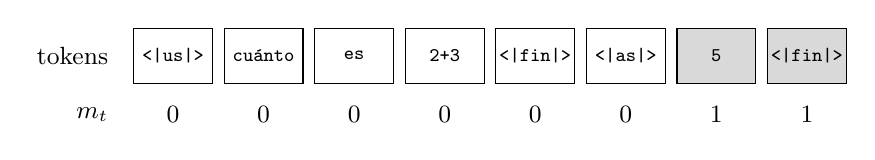
\begin{tikzpicture}[font=\small,
  t/.style={draw,minimum height=7mm,minimum width=10mm,inner sep=1pt,font=\scriptsize\ttfamily},
  on/.style={t,fill=black!15}]
  \foreach \txt/\st [count=\i] in {<|us|>/t,cuánto/t,es/t,2+3/t,<|fin|>/t,<|as|>/t,5/on,<|fin|>/on}{
    \node[\st] (n\i) at (1.15*\i,0) {\txt};
  }
  \foreach \v [count=\i] in {0,0,0,0,0,0,1,1}{
    \node[font=\small] at (1.15*\i,-0.75) {$\v$};
  }
  \node[anchor=east,font=\small] at (0.45,0) {tokens};
  \node[anchor=east,font=\small] at (0.45,-0.75) {$m_t$};
\end{tikzpicture}
\caption{Plantilla de chat de un turno (\texttt{us}: usuario; \texttt{as}: asistente) y su máscara. Solo puntúan el contenido de la respuesta y el token de fin que la cierra (sombreados).}
\label{fig:plantilla}
\end{figure}

En la inferencia, la aplicación construye la plantilla con todo el historial, añade $\langle\text{asistente}\rangle$ y deja que el modelo genere hasta emitir $\langle\mathrm{fin}\rangle$. Incluir el token de fin en la pérdida es imprescindible para que el modelo aprenda a terminar su turno: en la práctica del módulo, el modelo base no lo emite nunca y, tras 600 pasos de SFT, lo emite en el $99{,}4\,\%$ de los ejemplos de entrenamiento y en el $100\,\%$ de los de prueba.

\begin{observacion}
Los tokens especiales se añaden al vocabulario antes del ajuste (módulo~12) y sus vectores de \emph{embedding} se aprenden durante él. Por eso la plantilla forma parte del modelo: usar un modelo ajustado con una plantilla distinta de la suya degrada su comportamiento. Cada laboratorio usa su propio formato interno y no siempre lo publica; lo que documentan públicamente las API de Claude, Gemini y Grok es que los mensajes se envían como una lista de pares (rol, contenido).
\end{observacion}

\section{¿Cuántos datos hacen falta? La alineación superficial}

El preentrenamiento consume billones de tokens; el ajuste supervisado publicado usa entre miles y cientos de miles de diálogos. Zhou \emph{et al.}~\cite{zhou-lima} ajustaron un modelo LLaMa de 65\,000 millones de parámetros con solo 1000 pares instrucción--respuesta seleccionados con cuidado (LIMA); en una evaluación humana controlada, sus respuestas empataron con las de GPT-4 o fueron preferidas a ellas en el $43\,\%$ de los casos. De ahí la \emph{hipótesis de la alineación superficial}: casi todo el conocimiento del modelo se adquiere en el preentrenamiento, y el ajuste enseña sobre todo qué formato y qué estilo usar al interactuar con un usuario. En la misma línea, Dettmers \emph{et al.}~\cite[§1]{dettmers} observaron que un conjunto de 9000 diálogos de alta calidad (OASST1) daba mejores asistentes que una submuestra de 450\,000 ejemplos de FLAN~v2.

\begin{observacion}
Estas conclusiones proceden de evaluaciones concretas de calidad conversacional y no implican que los datos de SFT sean irrelevantes para todas las capacidades: tareas como el razonamiento matemático o la programación se benefician de muchos más ejemplos. La lección robusta es que la calidad y la diversidad de los datos pesan más que su cantidad.
\end{observacion}

\begin{lecturas}
\item Jurafsky y Martin~\cite{jm3}, §8.1 «Instruction Tuning», con §8.1.1 (datos) y §8.1.2 (evaluación).
\item CS336~\cite{cs336}, clase~15 «Alignment -- SFT/RLHF», y tarea~5~\cite[§4]{cs336a5}.
\item CS224N~\cite{cs224n}, clase~8 «Post-training».
\item Wei \emph{et al.}~\cite{wei-flan} (FLAN) y Sanh \emph{et al.}~\cite{sanh-t0} (T0).
\item Ouyang \emph{et al.}~\cite{ouyang}, §3.2 (datos) y §3.5 (modelos), y Zhou \emph{et al.}~\cite{zhou-lima}.
\end{lecturas}

\section*{Ejercicios del tema 2}
\addcontentsline{toc}{section}{Ejercicios del tema 2}

\begin{ejercicio}{1}{eje:2-base}
Explique por qué un modelo base, al recibir «p: capital de francia\textbackslash n r:», no responde «paris» aunque el dato esté en su texto de entrenamiento, y qué le enseña el ajuste supervisado.
\end{ejercicio}

\begin{ejercicio}{1}{eje:2-ignore}
¿Qué ocurre con una posición cuya etiqueta vale $-100$ en \texttt{cross\_entropy(\dots, ignore\_index=-100)}? ¿Por qué se usa también en las posiciones de relleno?
\end{ejercicio}

\begin{ejercicio}{2}{eje:2-mascara}
Una secuencia tiene 4 tokens de instrucción con pérdidas $2{,}1$; $1{,}8$; $0{,}9$; $1{,}1$ y 3 de respuesta con $0{,}6$; $0{,}2$; $0{,}4$. Calcule la pérdida media sin máscara y con máscara.
\end{ejercicio}

\begin{ejercicio}{1}{eje:2-tokenizar}
Se tienen dos ejemplos tokenizados. Ejemplo~1: instrucción $[5,9,2]$ y respuesta $[7,3,0]$. Ejemplo~2: instrucción $[4,8]$ y respuesta $[6,0]$. El índice~0 es el token de fin y el~1, el de relleno. Concatene instrucción y respuesta, rellene a la longitud máxima y construya \texttt{input\_\allowbreak ids} (la secuencia sin su último token), \texttt{labels} (la secuencia sin su primer token) y \texttt{response\_\allowbreak mask} (1 donde la etiqueta pertenece a la respuesta). ¿Cuántas posiciones puntúan en cada ejemplo?
\fuente{adaptado de Stanford CS336, primavera de 2025, tarea~5~\cite[§4.2]{cs336a5}, problema \texttt{tokenize\_\allowbreak prompt\_\allowbreak and\_\allowbreak output}.}
\end{ejercicio}

\begin{ejercicio}{2}{eje:2-microlote}
Un microlote tiene 2 secuencias de 5 posiciones, con log-probabilidades por token $(-2{,}0;\,-1{,}5;\,-0{,}5;\,-1{,}0;\,-0{,}1)$ y $(-1{,}2;\,-0{,}4;\,-0{,}2;\,-3{,}0;\,-3{,}0)$ y máscaras de respuesta $(0,0,1,1,1)$ y $(0,1,1,0,0)$. La pérdida del microlote es la suma enmascarada de $-\ln p$ dividida por el tamaño del microlote, por una constante $c=1$ y por el número de pasos de acumulación, $2$. Calcule esa pérdida y compárela con la media por token de respuesta, $J_{\mathrm{tok}}$.
\fuente{adaptado de Stanford CS336, primavera de 2025, tarea~5~\cite[§4.2]{cs336a5}, problemas \texttt{masked\_\allowbreak normalize} y \texttt{sft\_\allowbreak microbatch\_\allowbreak train\_\allowbreak step}.}
\end{ejercicio}

\begin{ejercicio}{1}{eje:2-empaquetar}
Se tienen tres ejemplos de 7, 5 y 9 tokens. Se añade un token de fin tras cada uno, se concatenan y se corta la cadena en trozos consecutivos de 5 tokens, descartando el último si está incompleto. ¿Cuántas secuencias se obtienen y cuántos tokens se pierden? Compárese con rellenar cada ejemplo, con su fin, hasta 10 tokens: ¿qué fracción de posiciones es útil en cada caso?
\fuente{adaptado de Stanford CS336, primavera de 2026, suplemento de la tarea~5~\cite[§4.2]{cs336a5s}, problema \texttt{data\_\allowbreak loading}.}
\end{ejercicio}

\begin{ejercicio}{3}{eje:2-multiturno}
Un diálogo alterna $K$ turnos de usuario $u^{(1)},\dots,u^{(K)}$ y $K$ respuestas del asistente $y^{(1)},\dots,y^{(K)}$, de longitudes $m_1,\dots,m_K$, en el orden $u^{(1)},y^{(1)},\dots,u^{(K)},y^{(K)}$. Con la máscara de la \cref{def:plantilla}, demuestre que
\[
\Lsft=-\frac{1}{\sum_k m_k}\sum_{k=1}^{K}\ln p_\theta\bigl(y^{(k)}\,\big|\,h^{(k)}\bigr),
\]
donde $h^{(k)}=(u^{(1)},y^{(1)},\dots,u^{(k)})$ es el historial que precede a la respuesta $k$ (se omiten los tokens de rol y de fin para simplificar). Interprete el resultado.
\end{ejercicio}

% =====================================================================
\chapter{Olvido catastrófico}
\label{tema:3}
% =====================================================================

Al ajustar todos los pesos con una tarea estrecha, el modelo pierde capacidades que tenía. Este tema define el fenómeno, lo analiza en un modelo cuadrático que puede resolverse a mano y deduce la penalización de la consolidación elástica de pesos (EWC) como aproximación bayesiana. El fenómeno se describió en redes conexionistas en el trabajo de McCloskey y Cohen~\cite{mccloskey}; EWC procede de Kirkpatrick \emph{et al.}~\cite{kirkpatrick}; la aproximación de Laplace sigue el §4.4 de Bishop~\cite{bishop}, y el análisis cuadrático de la penalización, el §7.1.1 de Goodfellow, Bengio y Courville~\cite{gbc}.

\section{El fenómeno}

\begin{definicion}[Olvido]\label{def:olvido}
Sean $\mathcal{L}_A$ la pérdida de una tarea antigua, $\theta_0$ unos parámetros que la resuelven y $\theta_B$ los parámetros obtenidos al ajustar $\theta_0$ con una tarea nueva de pérdida $\mathcal{L}_B$. El \emph{olvido} es el aumento $\mathcal{L}_A(\theta_B)-\mathcal{L}_A(\theta_0)$. Se habla de \emph{olvido catastrófico} cuando ese aumento es comparable al que tendría un modelo sin entrenar en la tarea~$A$.
\end{definicion}

McCloskey y Cohen~\cite{mccloskey} mostraron en 1989 que una red entrenada secuencialmente en dos tareas pierde casi por completo la primera al aprender la segunda, a diferencia de lo que ocurre en el aprendizaje humano. La causa es que los mismos parámetros codifican ambas tareas y el gradiente de $\mathcal{L}_B$ no tiene en cuenta cuánto importa cada parámetro para~$A$.

\begin{ejemplo}[El olvido en la práctica del módulo]\label{ej:olvido-practica}
La práctica mide la pérdida del mini-GPT sobre el texto de preentrenamiento antes y después del ajuste supervisado:
\begin{center}\small
\begin{tabular}{@{}lcc@{}}
\toprule
Modelo & Exactitud en prueba & Pérdida de texto (nats) \\
\midrule
Base & $0$ & $0{,}192$ \\
SFT completo ($\eta=10^{-3}$) & $0{,}300$ & $2{,}073$ \\
SFT con LoRA ($r=4$, $\eta=10^{-2}$) & $0{,}450$ & $5{,}058$ \\
LoRA con el adaptador desactivado & $0$ & $0{,}192$ \\
LoRA con repetición de texto & $0{,}475$ & $0{,}194$ \\
\bottomrule
\end{tabular}
\end{center}
La pérdida de texto de los modelos ajustados se dispara. Desactivar el adaptador LoRA devuelve exactamente el modelo base, porque la matriz $W$ no se ha modificado (\cref{tema:5}). Mezclar en cada paso una fracción de pérdida de preentrenamiento (repetición, \cref{def:replay}) conserva la tarea y casi no olvida.
\end{ejemplo}

\section{Un modelo cuadrático del compromiso}

\begin{proposicion}[Muelle hacia el modelo preentrenado]\label{prop:muelle}
Sean $a,\theta_0\in\R$ y $\lambda\ge 0$, y sea
\[
\mathcal{L}(\theta)=(\theta-a)^{2}+\lambda(\theta-\theta_0)^{2}.
\]
El único minimizador es $\theta^{\ast}=(a+\lambda\theta_0)/(1+\lambda)$. En él, el olvido medido como $(\theta^{\ast}-\theta_0)^{2}$ y el error en la tarea nueva $(\theta^{\ast}-a)^{2}$ valen
\[
(\theta^{\ast}-\theta_0)^{2}=\frac{(a-\theta_0)^{2}}{(1+\lambda)^{2}},\qquad (\theta^{\ast}-a)^{2}=\frac{\lambda^{2}(a-\theta_0)^{2}}{(1+\lambda)^{2}}.
\]
\end{proposicion}

\begin{proof}
$\mathcal{L}'(\theta)=2(\theta-a)+2\lambda(\theta-\theta_0)$ se anula si y solo si $\theta(1+\lambda)=a+\lambda\theta_0$. Como $\mathcal{L}''=2(1+\lambda)>0$, $\mathcal{L}$ es estrictamente convexa y el punto crítico es el mínimo global. Además, $\theta^{\ast}-\theta_0=(a-\theta_0)/(1+\lambda)$ y $\theta^{\ast}-a=\lambda(\theta_0-a)/(1+\lambda)$; elevando al cuadrado se obtienen las fórmulas.
\end{proof}

\begin{corolario}\label{cor:frontera}
Las distancias $\abs{\theta^{\ast}-\theta_0}$ y $\abs{\theta^{\ast}-a}$ suman $\abs{a-\theta_0}$ para todo $\lambda\ge 0$: $\theta^{\ast}$ recorre el segmento entre $a$ y $\theta_0$, desde $\theta^{\ast}=a$ ($\lambda=0$, olvido máximo) hasta $\theta^{\ast}\to\theta_0$ ($\lambda\to\infty$, ningún aprendizaje).
\end{corolario}

\begin{proof}
Por la proposición, $\abs{\theta^{\ast}-\theta_0}+\abs{\theta^{\ast}-a}=\frac{1+\lambda}{1+\lambda}\abs{a-\theta_0}$. Los límites se leen en la expresión de $\theta^{\ast}$.
\end{proof}

\begin{ejemplo}\label{ej:muelle}
Con $\theta_0=1$ y $a=3$, la \cref{prop:muelle} da $\theta^{\ast}=(3+\lambda)/(1+\lambda)$:
\begin{center}\small
\begin{tabular}{@{}cccc@{}}
\toprule
$\lambda$ & $\theta^{\ast}$ & Olvido $(\theta^{\ast}-1)^{2}$ & Error en la tarea $(\theta^{\ast}-3)^{2}$ \\
\midrule
$0$ & $3$ & $4$ & $0$ \\
$1$ & $2$ & $1$ & $1$ \\
$3$ & $1{,}5$ & $0{,}25$ & $2{,}25$ \\
\bottomrule
\end{tabular}
\end{center}
\end{ejemplo}

La penalización $\lambda(\theta-\theta_0)^{2}$ es la energía potencial de un muelle de constante $2\lambda$ anclado en $\theta_0$, y $\theta^{\ast}$ es el punto de equilibrio entre dos fuerzas lineales. El problema real tiene millones de parámetros, y no todos importan igual para la tarea antigua: conviene un muelle más rígido en los parámetros importantes. Esa es la idea de EWC.

\section{Consolidación elástica de pesos}

\subsection{Justificación bayesiana}

Sean $\mathcal{D}_A$ y $\mathcal{D}_B$ los datos de las dos tareas, condicionalmente independientes dado $\theta$. Por el teorema de Bayes,
\begin{equation}\label{eq:bayes-secuencial}
\ln p(\theta\mid\mathcal{D}_A,\mathcal{D}_B)=\ln p(\mathcal{D}_B\mid\theta)+\ln p(\theta\mid\mathcal{D}_A)-\ln p(\mathcal{D}_B\mid\mathcal{D}_A).
\end{equation}
El último término no depende de $\theta$. Toda la información sobre la tarea~$A$ está en la distribución a posteriori $p(\theta\mid\mathcal{D}_A)$, que no puede calcularse exactamente. La \emph{aproximación de Laplace}~\cite[§4.4]{bishop} la sustituye por una gaussiana centrada en su moda.

\begin{definicion}[Aproximación de Laplace]\label{def:laplace}
Sea $\theta_A$ un máximo de $g(\theta)=\ln p(\theta\mid\mathcal{D}_A)$ y sea $H_A=-\nabla^{2}g(\theta_A)$, definida positiva. La aproximación de Laplace es $p(\theta\mid\mathcal{D}_A)\approx\mathcal{N}(\theta;\theta_A,H_A^{-1})$, que se obtiene del desarrollo de Taylor de segundo orden $g(\theta)\approx g(\theta_A)-\frac12(\theta-\theta_A)\T H_A(\theta-\theta_A)$, en el que el término lineal se anula porque $\nabla g(\theta_A)=0$.
\end{definicion}

Sustituyendo en~\eqref{eq:bayes-secuencial}, maximizar la distribución a posteriori conjunta equivale aproximadamente a minimizar
\[
-\ln p(\mathcal{D}_B\mid\theta)+\tfrac12(\theta-\theta_A)\T H_A(\theta-\theta_A).
\]
Queda por estimar $H_A$, una matriz de $D\times D$ con $D$ del orden de millones.

\subsection{Información de Fisher}

\begin{definicion}[Información de Fisher]\label{def:fisher}
Sea $p_\theta$ una familia de distribuciones derivable en $\theta$. Su \emph{matriz de información de Fisher} es
\[
\Fis(\theta)=\E_{x\sim p_\theta}\bigl[\nabla_\theta\ln p_\theta(x)\,\nabla_\theta\ln p_\theta(x)\T\bigr].
\]
El vector $\nabla_\theta\ln p_\theta(x)$ se llama \emph{función de puntuación} (\emph{score}).
\end{definicion}

$\Fis(\theta)$ es semidefinida positiva por ser la esperanza de matrices de la forma $vv\T$. Solo requiere gradientes de primer orden.

\begin{proposicion}[Fisher como hessiano esperado]\label{prop:fisher-hess}
Supóngase que se pueden intercambiar derivada e integral. Entonces $\E_{x\sim p_\theta}[\nabla_\theta\ln p_\theta(x)]=0$ y
\[
\Fis(\theta)=-\E_{x\sim p_\theta}\bigl[\nabla^{2}_\theta\ln p_\theta(x)\bigr].
\]
\end{proposicion}

\begin{proof}
Como $\nabla\ln p_\theta=\nabla p_\theta/p_\theta$, se tiene $\E[\nabla\ln p_\theta]=\int\nabla p_\theta(x)\,dx=\nabla\int p_\theta(x)\,dx=\nabla 1=0$. Derivando de nuevo, $\nabla^{2}\ln p_\theta=\nabla^{2}p_\theta/p_\theta-\nabla\ln p_\theta\,\nabla\ln p_\theta\T$. Tomando esperanzas, el primer término da $\int\nabla^{2}p_\theta(x)\,dx=\nabla^{2}1=0$, de modo que $\E[\nabla^{2}\ln p_\theta]=-\Fis(\theta)$.
\end{proof}

Si $\mathcal{D}_A$ consta de $n$ ejemplos y la distribución a priori es plana, $H_A=-\sum_{i}\nabla^{2}\ln p_\theta(x_i)\big|_{\theta_A}$, y por la ley de los grandes números y la \cref{prop:fisher-hess} se aproxima por $n\,\Fis(\theta_A)$ cuando el modelo describe bien los datos. Kirkpatrick \emph{et al.} se quedan además con la diagonal, $F_i=\Fis_{ii}(\theta_A)$, que se estima promediando los cuadrados de las componentes del gradiente.

\begin{definicion}[EWC]\label{def:ewc}
Sean $\theta_A$ los parámetros tras la tarea~$A$ y $F_i$ la diagonal de su matriz de Fisher. La \emph{consolidación elástica de pesos} minimiza
\[
\mathcal{L}_{\mathrm{EWC}}(\theta)=\mathcal{L}_B(\theta)+\sum_{i=1}^{D}\frac{\lambda}{2}F_i\,(\theta_i-\theta_{A,i})^{2},
\]
donde $\lambda>0$ regula la importancia de la tarea antigua~\cite{kirkpatrick}.
\end{definicion}

Cada parámetro tiene su propio muelle, de constante $\lambda F_i$: los parámetros a los que la verosimilitud de la tarea~$A$ es sensible (Fisher grande) quedan rígidos y los demás pueden moverse libremente. La \cref{prop:muelle} es el caso de un solo parámetro en el que el coeficiente $\frac{\lambda}{2}F$ de EWC hace el papel del $\lambda$ de la proposición.

\section{Otros remedios}

\begin{definicion}[Repetición]\label{def:replay}
La \emph{repetición} (\emph{replay}) mezcla en cada paso ejemplos de la tarea antigua: con $\beta\in[0,1)$, se minimiza $(1-\beta)\mathcal{L}_B(\theta)+\beta\,\mathcal{L}_A(\theta)$.
\end{definicion}

Otros remedios habituales son una tasa de aprendizaje pequeña y pocas épocas, las técnicas de ULMFiT (\cref{tema:1}) y modificar pocos parámetros, como hacen los métodos del \cref{tema:4} y LoRA (\cref{tema:5}). El módulo~21 penalizará la divergencia de Kullback--Leibler entre el modelo ajustado y uno de referencia. Esa penalización actúa en el espacio de las distribuciones de salida, pero localmente coincide con un muelle en el espacio de parámetros cuya rigidez es la información de Fisher.

\begin{proposicion}[Desarrollo local de la divergencia KL]\label{prop:kl-fisher}
Bajo las hipótesis de la \cref{prop:fisher-hess}, y si $\ln p_\theta$ es tres veces derivable,
\[
D_{\mathrm{KL}}\bigl(p_{\theta_0}\,\big\|\,p_{\theta_0+\delta}\bigr)=\tfrac12\,\delta\T\Fis(\theta_0)\,\delta+O(\norm{\delta}^{3}).
\]
\end{proposicion}

\begin{proof}
Sea $k(\delta)=D_{\mathrm{KL}}(p_{\theta_0}\|p_{\theta_0+\delta})=\E_{x\sim p_{\theta_0}}[\ln p_{\theta_0}(x)-\ln p_{\theta_0+\delta}(x)]$. Se tiene $k(0)=0$. Su gradiente en $\delta=0$ es $-\E_{p_{\theta_0}}[\nabla\ln p_{\theta_0}]=0$ por la \cref{prop:fisher-hess}, y su hessiano en $\delta=0$ es $-\E_{p_{\theta_0}}[\nabla^{2}\ln p_{\theta_0}]=\Fis(\theta_0)$ por la misma proposición. El desarrollo de Taylor de segundo orden con resto de orden tres da el enunciado.
\end{proof}

\begin{lecturas}
\item McCloskey y Cohen~\cite{mccloskey}, descripción original de la interferencia catastrófica.
\item Kirkpatrick \emph{et al.}~\cite{kirkpatrick}, sección sobre la consolidación elástica de pesos y su justificación bayesiana.
\item Bishop~\cite{bishop}, §4.4 «The Laplace Approximation».
\item Goodfellow, Bengio y Courville~\cite{gbc}, §7.1.1 «$L^2$ Parameter Regularization».
\end{lecturas}

\section*{Ejercicios del tema 3}
\addcontentsline{toc}{section}{Ejercicios del tema 3}

\begin{ejercicio}{1}{eje:3-remedios}
Enumere cuatro remedios contra el olvido catastrófico y clasifíquelos según actúen sobre los datos, sobre la pérdida, sobre el optimizador o sobre los parámetros que se entrenan. ¿Cuál de ellos permite recuperar \emph{exactamente} el modelo base después del ajuste, y por qué?
\end{ejercicio}

\begin{ejercicio}{3}{eje:3-muelle}
En el modelo cuadrático con $\theta_0=1$, tarea $(\theta-3)^{2}$ y muelle $\lambda(\theta-\theta_0)^{2}$, deduzca $\theta^{\ast}(\lambda)$ sin usar la \cref{prop:muelle} y calcule $\theta^{\ast}$, el olvido $(\theta^{\ast}-1)^{2}$ y el error en la tarea para $\lambda=2$. ¿Qué ocurre cuando $\lambda\to\infty$?
\end{ejercicio}

\begin{ejercicio}{2}{eje:3-ewc}
Un modelo tiene dos parámetros, con $\theta_A=(1,1)$ tras la tarea antigua y diagonal de Fisher $F=(4;\,0{,}25)$. La tarea nueva tiene pérdida $\mathcal{L}_B(\theta)=(\theta_1-3)^{2}+(\theta_2-3)^{2}$. Con $\lambda=2$, minimice $\mathcal{L}_{\mathrm{EWC}}$ y calcule la penalización $\frac12\sum_iF_i(\theta^{\ast}_i-1)^{2}$, que aproxima el aumento de la pérdida antigua, y el error en la tarea nueva $\mathcal{L}_B(\theta^{\ast})$. ¿Qué parámetro se mueve más y por qué?
\end{ejercicio}

\begin{ejercicio}{2}{eje:3-replay}
Con un solo parámetro, $\mathcal{L}_B(\theta)=(\theta-3)^{2}$ y $\mathcal{L}_A(\theta)=(\theta-1)^{2}$, la repetición con proporción $\beta$ minimiza $(1-\beta)\mathcal{L}_B+\beta\mathcal{L}_A$. (a) Halle $\theta^{\ast}(\beta)$ y evalúelo para $\beta=0{,}25$. (b) Compruebe que coincide con el muelle de la \cref{prop:muelle} para $\lambda=\beta/(1-\beta)$.
\end{ejercicio}

\begin{ejercicio}{2}{eje:3-fisher}
Sea una variable de Bernoulli parametrizada por su logit, $p_z(1)=\sigma(z)$ y $p_z(0)=1-\sigma(z)$, con $\sigma$ la función logística. (a) Calcule la función de puntuación y demuestre que $\Fis(z)=\sigma(z)(1-\sigma(z))$. (b) Evalúela en $z=0$ y en $z=\ln 9$. (c) Si estos fueran dos parámetros de un modelo, ¿cuál quedaría más rígido con EWC?
\end{ejercicio}

\begin{ejercicio}{3}{eje:3-gbc}
Sea $\mathcal{L}_B(\theta)=\frac12(\theta-\theta_B)\T H(\theta-\theta_B)$, con $H$ simétrica definida positiva de autovalores $h_1,\dots,h_D$ y autovectores ortonormales $q_1,\dots,q_D$, y sea la penalización $\frac{\lambda}{2}\norm{\theta-\theta_0}^{2}$. (a) Demuestre que el minimizador es $\theta^{\ast}=(H+\lambda I)^{-1}(H\theta_B+\lambda\theta_0)$. (b) Demuestre que la componente de $\theta^{\ast}-\theta_0$ en la dirección $q_i$ es la de $\theta_B-\theta_0$ multiplicada por $h_i/(h_i+\lambda)$. (c) Evalúe $\theta^{\ast}$ con $H=\diag(10;\,0{,}1)$, $\lambda=1$, $\theta_0=0$ y $\theta_B=(1,1)$, e interprete el resultado.
\fuente{adaptado de Goodfellow, Bengio y Courville~\cite{gbc}, §7.1.1 (análisis cuadrático de la penalización $L^{2}$, aquí centrada en $\theta_0$ en lugar de en el origen).}
\end{ejercicio}

% =====================================================================
\chapter{Ajuste eficiente en parámetros}
\label{tema:4}
% =====================================================================

El ajuste completo de un modelo de $D$ parámetros produce, para cada tarea, una copia de $D$ parámetros y exige guardar durante el entrenamiento el estado del optimizador de todos ellos. Los métodos de \emph{ajuste eficiente en parámetros} (PEFT, del inglés \emph{parameter-efficient fine-tuning}) congelan el modelo preentrenado y entrenan un número pequeño de parámetros nuevos. Este tema presenta los adaptadores, el ajuste de \emph{prompt} y de prefijo, y la noción de dimensión intrínseca que explica por qué bastan tan pocos parámetros. Se sigue el §8.2 de Jurafsky y Martin~\cite{jm3}, la clase~9 de CS224N~\cite{cs224n} y los artículos originales~\cite{houlsby,lester,li-liang,li-intrinsic,aghajanyan}; LoRA, el método más usado, ocupa el \cref{tema:5}.

\section{Planteamiento}

\begin{definicion}[Ajuste eficiente en parámetros]\label{def:peft}
Sea $\theta_0\in\R^{D}$ un modelo preentrenado. Un método PEFT define una familia de modelos $f_{\theta_0,\varphi}$ con parámetros nuevos $\varphi\in\R^{P}$, $P\ll D$, tal que existe $\varphi_0$ con $f_{\theta_0,\varphi_0}=f_{\theta_0}$, y entrena solo $\varphi$, partiendo de $\varphi_0$ o de un valor próximo, con $\theta_0$ congelado.
\end{definicion}

Los métodos se agrupan en tres familias: \emph{aditivos}, que añaden módulos o vectores nuevos (adaptadores, ajuste de \emph{prompt} y de prefijo); \emph{selectivos}, que entrenan un subconjunto de los parámetros existentes (la sonda lineal del \cref{tema:1} es el caso extremo), y de \emph{reparametrización}, que escriben la actualización $\Delta\theta$ como función de pocos parámetros (subespacios aleatorios, \cref{sec:intrinseca}, y LoRA, \cref{tema:5}).

\begin{proposicion}[Memoria del entrenamiento]\label{prop:memoria-peft}
Con precisión mixta y Adam, el ajuste completo requiere unos $16D$ bytes para pesos, gradientes y estado del optimizador (módulo~17). Con un método PEFT y el modelo base en bf16, la memoria es de unos $2D+16P$ bytes, sin contar las activaciones.
\end{proposicion}

\begin{proof}
En el ajuste completo, cada parámetro ocupa 2 bytes de peso en bf16, 2 de gradiente, 4 de copia maestra en fp32 y 8 de los dos momentos de Adam en fp32: 16 bytes. En un método PEFT los $D$ parámetros congelados solo necesitan su peso en bf16 (2 bytes): no tienen gradiente ni estado de Adam. Los $P$ parámetros entrenables necesitan los 16 bytes completos.
\end{proof}

Con $D=7\cdot 10^{9}$ y $P=2\cdot 10^{7}$, la memoria baja de $112$~GB a $14+0{,}32=14{,}32$~GB. Además, cada tarea se almacena con $P$ parámetros en lugar de $D$, y un mismo modelo base puede servir muchas tareas cambiando solo $\varphi$.

\section{Adaptadores}

\begin{definicion}[Adaptador]\label{def:adaptador}
Sea $h\in\R^{d}$ la salida de una subcapa de un Transformer. Un \emph{adaptador} con dimensión de cuello $m\ll d$ calcula
\[
a(h)=h+W_{\uparrow}\,g\bigl(W_{\downarrow}h+b_{\downarrow}\bigr)+b_{\uparrow},\qquad W_{\downarrow}\in\R^{m\times d},\ W_{\uparrow}\in\R^{d\times m},
\]
con $g$ una no linealidad. Houlsby \emph{et al.}~\cite{houlsby} insertan dos adaptadores por capa, tras la subcapa de atención y tras la red de alimentación hacia delante, y entrenan además los parámetros de normalización de capa.
\end{definicion}

\begin{figure}[h]
\centering
\begin{tikzpicture}[>={Stealth[length=2mm]},font=\small,
  caja/.style={draw,thick,minimum height=7mm,minimum width=30mm,align=center}]
  \node (in) at (0,0) {$h\in\R^{d}$};
  \node[caja] (d) at (0,1.2) {$W_{\downarrow}$: $d\to m$};
  \node[caja] (g) at (0,2.3) {no linealidad $g$};
  \node[caja] (u) at (0,3.4) {$W_{\uparrow}$: $m\to d$};
  \node[draw,thick,circle,inner sep=1pt] (s) at (0,4.5) {$+$};
  \node (out) at (0,5.4) {$a(h)\in\R^{d}$};
  \draw[->] (in) -- (d);
  \draw[->] (d) -- (g);
  \draw[->] (g) -- (u);
  \draw[->] (u) -- (s);
  \draw[->] (s) -- (out);
  \draw[->] (in.east) -- ++(1.9,0) |- node[pos=0.25,right] {identidad} (s.east);
\end{tikzpicture}
\caption{Adaptador con cuello de botella. Si $W_{\uparrow}$ y $b_{\uparrow}$ son nulos, el adaptador es la identidad.}
\label{fig:adaptador}
\end{figure}

\begin{proposicion}\label{prop:adaptador}
Un adaptador tiene $2md+m+d$ parámetros. Si se inicializa con $W_{\uparrow}=0$ y $b_{\uparrow}=0$, entonces $a(h)=h$ para todo $h$, de modo que el modelo con adaptadores coincide al principio con el preentrenado.
\end{proposicion}

\begin{proof}
$W_{\downarrow}$ y $W_{\uparrow}$ aportan $md$ parámetros cada una; $b_{\downarrow}\in\R^{m}$ y $b_{\uparrow}\in\R^{d}$, $m+d$. Con $W_{\uparrow}=0$ y $b_{\uparrow}=0$, el sumando $W_{\uparrow}g(\cdot)+b_{\uparrow}$ es nulo.
\end{proof}

Houlsby \emph{et al.} usan una inicialización \emph{casi} nula, de modo que el adaptador es casi la identidad, y obtienen en GLUE resultados a menos de un $0{,}4\,\%$ de los del ajuste completo añadiendo un $3{,}6\,\%$ de parámetros por tarea~\cite{houlsby}.

\begin{observacion}[Latencia]
Los adaptadores añaden capas que se ejecutan en serie y no pueden fusionarse con los pesos originales, porque contienen una no linealidad. Hu \emph{et al.}~\cite[§3]{hu-lora} midieron aumentos de la latencia de inferencia superiores al $30\,\%$ con secuencias cortas y lotes pequeños. LoRA evita este problema (\cref{tema:5}).
\end{observacion}

\section{Ajuste de \emph{prompt} y de prefijo}

\begin{definicion}[Ajuste de \emph{prompt}]\label{def:prompt-tuning}
Sea $E\in\R^{T\times d}$ la matriz de \emph{embeddings} de una entrada. El \emph{ajuste de prompt} antepone $p$ vectores entrenables $P_e\in\R^{p\times d}$ y alimenta el modelo congelado con $[P_e;E]\in\R^{(p+T)\times d}$. Tiene $pd$ parámetros~\cite{lester}.
\end{definicion}

Los vectores de $P_e$ no tienen por qué corresponder a ningún token del vocabulario: forman un \emph{prompt continuo} (\emph{soft prompt}). Lester \emph{et al.}~\cite{lester} observaron que la diferencia con el ajuste completo disminuye con la escala y prácticamente desaparece en modelos de unos $10^{10}$ parámetros.

\begin{definicion}[Ajuste de prefijo]\label{def:prefix}
El \emph{ajuste de prefijo} antepone, en cada una de las $L$ capas, $p$ claves y $p$ valores entrenables, $P_K^{l},P_V^{l}\in\R^{p\times d}$, a las claves y valores calculados a partir de la entrada. Tiene $2Lpd$ parámetros. Para estabilizar el entrenamiento, Li y Liang~\cite{li-liang} reparametrizan los prefijos mediante una pequeña red que se descarta al terminar; con ello entrenan en torno al $0{,}1\,\%$ de los parámetros.
\end{definicion}

El efecto de un prefijo sobre la atención admite una descripción exacta.

\begin{teorema}[El prefijo interpola la atención]\label{teo:prefijo}
Sean $q\in\R^{d}$ una consulta, $K,V\in\R^{T\times d}$ las claves y valores de la entrada y $P_K,P_V\in\R^{p\times d}$ los del prefijo. Escríbase $\mathrm{At}(q,K,V)=\softmax(Kq/\sqrt{d})\T V$. Entonces
\[
\mathrm{At}\bigl(q,[P_K;K],[P_V;V]\bigr)=\bigl(1-\mu(q)\bigr)\,\mathrm{At}(q,K,V)+\mu(q)\,\mathrm{At}(q,P_K,P_V),
\]
con
\[
\mu(q)=\frac{S_P}{S_P+S_K},\qquad S_P=\sum_{j=1}^{p}e^{(P_K)_j\cdot q/\sqrt{d}},\quad S_K=\sum_{i=1}^{T}e^{k_i\cdot q/\sqrt{d}}.
\]
\end{teorema}

\begin{proof}
Sean $a_i=e^{k_i\cdot q/\sqrt d}$ y $b_j=e^{(P_K)_j\cdot q/\sqrt d}$. La atención sobre la concatenación es
\[
\frac{\sum_j b_j(P_V)_j+\sum_i a_iv_i}{S_P+S_K}
=\frac{S_P}{S_P+S_K}\cdot\frac{\sum_j b_j(P_V)_j}{S_P}+\frac{S_K}{S_P+S_K}\cdot\frac{\sum_i a_iv_i}{S_K}.
\]
Los dos cocientes de la derecha son, por definición de la softmax, $\mathrm{At}(q,P_K,P_V)$ y $\mathrm{At}(q,K,V)$, y $S_K/(S_P+S_K)=1-\mu(q)$.
\end{proof}

\begin{corolario}\label{cor:prefijo}
El ajuste de prefijo no altera los pesos relativos de atención entre las posiciones de la entrada: solo mezcla la salida original con un vector que depende de la consulta, con una proporción $\mu(q)\in(0,1)$.
\end{corolario}

Esta lectura, que relaciona el ajuste de prefijo con los adaptadores, se desarrolla en He \emph{et al.}~\cite{he-unified}.

\section{Dimensión intrínseca}\label{sec:intrinseca}

¿Por qué basta con ajustar una fracción mínima de los parámetros? Li \emph{et al.}~\cite{li-intrinsic} propusieron medir la dimensión efectiva de un problema de optimización restringiendo el entrenamiento a un subespacio aleatorio.

\begin{definicion}[Subespacio aleatorio y dimensión intrínseca]\label{def:intrinseca}
Sean $\theta_0\in\R^{D}$ y $P\in\R^{D\times d'}$ una matriz aleatoria fija. Se entrena solo $z\in\R^{d'}$, inicializado en $0$, con la reparametrización $\theta=\theta_0+Pz$. La \emph{dimensión intrínseca} $d_{90}$ de una tarea es el menor $d'$ con el que se alcanza el $90\,\%$ del rendimiento del ajuste completo~\cite[§3]{aghajanyan}.
\end{definicion}

\begin{proposicion}[Gradiente en el subespacio]\label{prop:grad-subespacio}
Si $\mathcal{L}$ es derivable, $\nabla_z\mathcal{L}(\theta_0+Pz)=P\T\,\nabla_\theta\mathcal{L}(\theta)\big|_{\theta=\theta_0+Pz}$.
\end{proposicion}

\begin{proof}
La aplicación $z\mapsto\theta_0+Pz$ es afín con jacobiana $P$. Por la regla de la cadena (módulo~4), $\nabla_z\mathcal{L}=P\T\nabla_\theta\mathcal{L}$.
\end{proof}

Aghajanyan \emph{et al.}~\cite{aghajanyan} estimaron la dimensión intrínseca del ajuste de modelos de lenguaje preentrenados, usando para $P$ la transformada Fastfood, que evita almacenar una matriz densa de $D\times d'$. Sus tres resultados principales son:
\begin{enumerate}
  \item con RoBERTa-Large, unos 200 parámetros bastan para alcanzar el $90\,\%$ del rendimiento del ajuste completo en la tarea MRPC~\cite[§4.2]{aghajanyan};
  \item la dimensión intrínseca disminuye a lo largo del preentrenamiento y es menor en los modelos con más parámetros~\cite[§5.1 y~§5.2]{aghajanyan};
  \item una cota de generalización basada en compresión depende de la dimensión intrínseca y no del número total de parámetros: con $n$ ejemplos, el error de generalización es $O(\sqrt{d_{90}/n})$, para modelos entrenados en el subespacio~\cite[§5.3]{aghajanyan}.
\end{enumerate}

\begin{observacion}
El segundo resultado explica en parte la paradoja de que los modelos mayores se ajusten con menos datos: el preentrenamiento comprime el problema de adaptación. Hu \emph{et al.} formularon a partir de aquí la hipótesis que motiva LoRA~\cite[§1 y~§4.1]{hu-lora}: si el ajuste vive en un subespacio de dimensión pequeña, también la actualización de cada matriz de pesos debe tener un \emph{rango intrínseco} bajo. LoRA no fija las direcciones al azar: aprende la mejor base de rango $r$.
\end{observacion}

\begin{lecturas}
\item Jurafsky y Martin~\cite{jm3}, §8.2 «Parameter Efficient Fine Tuning».
\item CS224N~\cite{cs224n}, clase~9 «Efficient Adaptation (Prompting + PEFT)».
\item Houlsby \emph{et al.}~\cite{houlsby}, sección sobre los adaptadores y su inicialización.
\item Lester \emph{et al.}~\cite{lester} y Li y Liang~\cite{li-liang}.
\item Aghajanyan \emph{et al.}~\cite{aghajanyan}, §3 (definición), §4 (resultados) y §5 (relación con el preentrenamiento y la generalización).
\end{lecturas}

\section*{Ejercicios del tema 4}
\addcontentsline{toc}{section}{Ejercicios del tema 4}

\begin{ejercicio}{1}{eje:4-congelar}
Sobre un cuerpo preentrenado con representaciones de dimensión $h=768$ y unos $1{,}1\cdot 10^{8}$ parámetros se coloca una cabeza lineal de 2 clases con sesgo. Se congelan todos los parámetros anteriores a la cabeza. (a) ¿Cuántos parámetros se entrenan y qué fracción del total representan? (b) ¿A qué familia de métodos PEFT pertenece este procedimiento? (c) ¿Cabe esperar más o menos exactitud que con el ajuste completo? Razone en qué casos la diferencia sería pequeña.
\fuente{adaptado de Zhang \emph{et al.}~\cite{d2l}, §14.2, ejercicio~3.}
\end{ejercicio}

\begin{ejercicio}{2}{eje:4-adaptadores}
Un Transformer de 12 capas con $d=768$ y unos $1{,}1\cdot 10^{8}$ parámetros lleva dos adaptadores por capa con $m=64$ (se ignoran los parámetros de normalización). (a) Calcule los parámetros de los adaptadores y su porcentaje respecto al modelo. (b) Compare el almacenamiento necesario para 20 tareas con adaptadores y con 20 copias ajustadas por completo.
\end{ejercicio}

\begin{ejercicio}{2}{eje:4-prefijo}
Un modelo tiene $L=24$ capas y $d=1024$. Calcule los parámetros entrenables del ajuste de \emph{prompt} y del ajuste de prefijo con $p=20$ vectores (sin contar la red de reparametrización) y el cociente entre ambos.
\end{ejercicio}

\begin{ejercicio}{2}{eje:4-subespacio}
Sean $D=3$, $\theta_0=(1,0,2)$, $P=(1,2,-1)\T$ (de modo que $d'=1$) y la pérdida $\mathcal{L}(\theta)=\norm{\theta-\theta^{\star}}^{2}$ con $\theta^{\star}=(2,3,1)$. (a) Halle el $z$ óptimo y el $\theta$ correspondiente. (b) Calcule la pérdida que queda y compárela con la del ajuste completo. (c) Compruebe la \cref{prop:grad-subespacio} en $z=0$.
\end{ejercicio}

\begin{ejercicio}{3}{eje:4-proyeccion}
En la reparametrización $\theta=\theta_0+Pz$: (a) demuestre que el conjunto de modelos alcanzables es el subespacio afín $\theta_0+\Col(P)$, de dimensión $\rango P$; (b) demuestre que un paso de descenso de gradiente en $z$ con tasa $\eta$ desplaza $\theta$ en $-\eta PP\T\nabla_\theta\mathcal{L}$; (c) si las columnas de $P$ son ortonormales, demuestre que ese desplazamiento es la proyección ortogonal sobre $\Col(P)$ del paso de descenso de gradiente del ajuste completo.
\end{ejercicio}

% =====================================================================
\chapter{LoRA: adaptación de bajo rango}
\label{tema:5}
% =====================================================================

LoRA (\emph{low-rank adaptation}) congela cada matriz preentrenada y aprende solo una corrección de rango bajo, escrita como producto de dos matrices delgadas. Es hoy el método PEFT más usado porque no añade latencia de inferencia y su análisis se reduce al álgebra lineal del módulo~3. Este tema sigue el artículo original de Hu \emph{et al.}~\cite[§4 y~§7]{hu-lora}, el teorema de Eckart y Young~\cite{eckart-young} en la forma del módulo~3 y de Deisenroth, Faisal y Ong~\cite[§4.6]{mml}, y la clase invitada sobre LoRA del curso CS224N~\cite{cs224n}.

\section{Definición y número de parámetros}

\begin{definicion}[LoRA]\label{def:lora}
Sea $W\in\R^{d\times k}$ una matriz preentrenada de una capa lineal $h=Wx$, con $x\in\R^{k}$. Sean $r\ll\min(d,k)$ el \emph{rango}, $\alpha>0$ un hiperparámetro de escala y $s=\alpha/r$. LoRA sustituye la capa por
\[
h=Wx+s\,BAx,\qquad A\in\R^{r\times k},\ B\in\R^{d\times r},
\]
con $W$ congelada y $A$, $B$ entrenables. Se inicializa $A$ con entradas gaussianas y $B=0$~\cite[§4.1]{hu-lora}. La matriz efectiva es $W'=W+s\,BA$.
\end{definicion}

\begin{figure}[h]
\centering
\begin{tikzpicture}[>={Stealth[length=2mm]},font=\small,
  caja/.style={draw,thick,minimum height=8mm,minimum width=24mm,align=center}]
  \node (x) at (0,0) {$x\in\R^{k}$};
  \node[caja] (W) at (3.6,0.9) {$W$ congelada\\ $d\times k$};
  \node[caja] (A) at (3.0,-0.9) {$A$ entrenable\\ $r\times k$};
  \node[caja] (B) at (6.2,-0.9) {$B$ entrenable\\ $d\times r$, $B_0=0$};
  \node[draw,thick,circle,inner sep=1pt] (s) at (8.6,0) {$+$};
  \node (h) at (10.7,0) {$h\in\R^{d}$};
  \draw[->] (x) |- (W);
  \draw[->] (x) |- (A);
  \draw[->] (A) -- node[above] {$\R^{r}$} (B);
  \draw[->] (W) -| (s);
  \draw[->] (B) -| node[pos=0.25,below] {$\times s$} (s);
  \draw[->] (s) -- (h);
\end{tikzpicture}
\caption{Capa lineal con LoRA. La entrada atraviesa la matriz congelada y, en paralelo, el cuello de dimensión $r$ formado por $A$ y $B$. Como $B$ empieza en cero, al principio $h=Wx$.}
\label{fig:lora}
\end{figure}

\begin{proposicion}[Parámetros y coste]\label{prop:lora-param}
LoRA entrena $r(d+k)$ parámetros por matriz, una fracción $r(d+k)/(dk)=r(1/d+1/k)$ de los $dk$ del ajuste completo. Calcular $s\,B(Ax)$ cuesta $2r(d+k)$ operaciones más un escalado, frente a las $2dk$ de $Wx$, y nunca requiere formar $BA$.
\end{proposicion}

\begin{proof}
$A$ tiene $rk$ entradas y $B$, $dr$. El producto $Ax$ es $(r\times k)(k\times 1)$ y cuesta $2rk$ operaciones (módulo~17, tema~1); $B(Ax)$ es $(d\times r)(r\times 1)$ y cuesta $2dr$.
\end{proof}

\begin{table}[h]
\centering\small
\caption{Parámetros entrenables de LoRA en una matriz.}\label{tab:lora}
\begin{tabular}{@{}lrrrr@{}}
\toprule
Matriz & $r$ & Completo $dk$ & LoRA $r(d+k)$ & Fracción \\
\midrule
$64\times 64$ & 4 & $4096$ & $512$ & $12{,}5\,\%$ \\
$768\times 768$ & 4 & $589\,824$ & $6144$ & $1{,}04\,\%$ \\
$4096\times 4096$ & 8 & $16\,777\,216$ & $65\,536$ & $0{,}39\,\%$ \\
$4096\times 4096$ & 16 & $16\,777\,216$ & $131\,072$ & $0{,}78\,\%$ \\
\bottomrule
\end{tabular}
\end{table}

\begin{ejemplo}[Una capa LoRA a mano]\label{ej:lora-mano}
Sean $W=I_2$, $B=(1,2)\T$, $A=(0{,}5;\,-1)$, $r=1$ y $\alpha=2$, de modo que $s=2$. Entonces
\[
BA=\begin{pmatrix}0{,}5&-1\\1&-2\end{pmatrix},\qquad W'=I+2BA=\begin{pmatrix}2&-2\\2&-3\end{pmatrix}.
\]
Para $x=(1,0)$: $Ax=0{,}5$, $B(Ax)=(0{,}5;\,1)$ y $h=(1,0)+2\cdot(0{,}5;\,1)=(2,2)$, que coincide con $W'x$.
\end{ejemplo}

En el mini-GPT de la práctica ($d=64$, red de alimentación de dimensión 256, 2 bloques), LoRA con $r=4$ en las cuatro matrices de atención ($64\times 64$) y las dos de la red de alimentación ($64\times 256$ y $256\times 64$) de cada bloque entrena $2\cdot(4\cdot 512+2\cdot 1280)=9216$ parámetros, el $8{,}57\,\%$ de los $107\,520$ del modelo. En GPT-3 de 175\,000 millones de parámetros, Hu \emph{et al.} redujeron los parámetros entrenables unas $10\,000$ veces y la memoria de GPU unas 3 veces respecto al ajuste completo con Adam; con $r=4$ en $W_Q$ y $W_V$, el punto de control pasó de unos 350~GB a unos 35~MB~\cite[§4.2]{hu-lora}.

\begin{proposicion}[Fusión]\label{prop:fusion}
Tras el entrenamiento, sustituir $W$ por $W'=W+s\,BA$ produce la misma función que la capa LoRA y el mismo coste de inferencia que la capa original.
\end{proposicion}

\begin{proof}
Por la distributividad del producto de matrices, $W'x=Wx+s\,(BA)x=Wx+s\,B(Ax)$ para todo $x$. $W'$ tiene la misma forma $d\times k$ que $W$, luego $W'x$ cuesta $2dk$ operaciones, como $Wx$.
\end{proof}

Así, LoRA no añade latencia de inferencia, a diferencia de los adaptadores del \cref{tema:4}. Sin fusionar, en cambio, un mismo modelo base puede servir muchos adaptadores pequeños e intercambiarlos en cada petición.

\section{Rango de la corrección}

\begin{proposicion}[Cota de rango]\label{prop:rango}
Para todo $A\in\R^{r\times k}$ y $B\in\R^{d\times r}$, $\rango(BA)\le r$.
\end{proposicion}

\begin{proof}
Para todo $x\in\R^{k}$, $(BA)x=B(Ax)$ es una combinación lineal de las $r$ columnas de $B$ con coeficientes las componentes de $Ax\in\R^{r}$. Luego $\img(BA)\subseteq\img(B)=\Col(B)$, que está generado por $r$ vectores y tiene dimensión a lo sumo~$r$. El rango es la dimensión de la imagen.
\end{proof}

\begin{proposicion}[Recíproco]\label{prop:factorizacion}
Toda matriz $M\in\R^{d\times k}$ con $\rango M\le r$ puede escribirse como $M=BA$ con $B\in\R^{d\times r}$ y $A\in\R^{r\times k}$.
\end{proposicion}

\begin{proof}
Sea $M=\sum_{i=1}^{\rho}\sigma_iu_iv_i\T$ la SVD reducida de $M$, con $\rho=\rango M\le r$ (módulo~3). Tómense como columnas de $B$ los vectores $\sigma_1u_1,\dots,\sigma_\rho u_\rho$, completados con $r-\rho$ columnas nulas, y como filas de $A$ los vectores $v_1\T,\dots,v_\rho\T$, completados con $r-\rho$ filas nulas. Entonces $BA=\sum_{i=1}^{\rho}\sigma_iu_iv_i\T=M$.
\end{proof}

\begin{corolario}\label{cor:representables}
El conjunto de correcciones que LoRA de rango $r$ puede representar es exactamente $\{\Delta W\in\R^{d\times k}:\rango\Delta W\le r\}$. Si $r<\min(d,k)$, ninguna corrección de rango completo es representable.
\end{corolario}

\section{Gradientes e inicialización}

\begin{proposicion}[Gradientes de LoRA]\label{prop:grad-lora}
Sea $h=Wx+s\,BAx$ y sea $G=\partial\mathcal{L}/\partial h\in\R^{d}$ el gradiente que llega a la salida. Entonces
\[
\frac{\partial\mathcal{L}}{\partial B}=s\,G\,(Ax)\T\in\R^{d\times r},\qquad
\frac{\partial\mathcal{L}}{\partial A}=s\,B\T G\,x\T\in\R^{r\times k}.
\]
Con un lote, se suman las contribuciones de cada ejemplo.
\end{proposicion}

\begin{proof}
Se usa la regla del módulo~4: si $h=Mz$ con $z$ fijo, entonces $\partial\mathcal{L}/\partial M=Gz\T$. (i) Respecto a $B$, $h$ depende de $B$ a través de $s\,B(Ax)$, que es de la forma $Mz$ con $M=B$ y $z=s\,Ax$; luego $\partial\mathcal{L}/\partial B=G\,(s\,Ax)\T$. (ii) Respecto a $A$, sea $c=Ax\in\R^{r}$. Como $h$ depende de $c$ a través de $s\,Bc$, se tiene $\partial\mathcal{L}/\partial c=s\,B\T G$. Y como $c=Ax$ es de la forma $Mz$ con $M=A$ y $z=x$, $\partial\mathcal{L}/\partial A=(s\,B\T G)\,x\T$.
\end{proof}

\begin{corolario}[Inicialización]\label{cor:init}
Con $B=0$ y $A$ aleatoria:
\begin{enumerate}
  \item $BA=0$ y el modelo ajustado empieza siendo exactamente el modelo base;
  \item en el primer paso $\partial\mathcal{L}/\partial A=0$, pero $\partial\mathcal{L}/\partial B=s\,G(Ax)\T\ne 0$ si $G\ne 0$ y $Ax\ne 0$, de modo que $B$ deja de ser nula y, desde el segundo paso, también $A$ recibe gradiente.
\end{enumerate}
En cambio, $(A,B)=(0,0)$ es un punto fijo del descenso de gradiente (\cref{eje:5-init}).
\end{corolario}

La elección simétrica, $A=0$ con $B$ aleatoria, también empieza en el modelo base y también permite aprender; el convenio del artículo original es $B=0$.

\section{La escala \texorpdfstring{$\alpha/r$}{alpha/r}}

\begin{proposicion}[Adam es invariante a la escala del gradiente]\label{prop:adam-escala}
Sea el optimizador Adam con $\varepsilon=0$ (módulo~7). Si se multiplican todos los gradientes por una constante $c>0$, la sucesión de actualizaciones de los parámetros no cambia.
\end{proposicion}

\begin{proof}
Con gradientes $cg_t$, los momentos pasan a ser $m'_t=c\,m_t$ y $v'_t=c^{2}v_t$, por ser medias móviles exponenciales lineales en $g_t$ y en $g_t^{2}$ respectivamente; las correcciones de sesgo no dependen de $c$. La actualización es $\eta\,\hat m'_t/\sqrt{\hat v'_t}=\eta\,c\,\hat m_t/(c\sqrt{\hat v_t})=\eta\,\hat m_t/\sqrt{\hat v_t}$.
\end{proof}

Por la \cref{prop:grad-lora}, el gradiente de $B$ es proporcional a $s$. Por la \cref{prop:adam-escala}, la actualización $\Delta B$ del primer paso no depende de $s$, y la variación de la función, $s\,\Delta B\,A\,x$, es proporcional a $s$. El factor $s=\alpha/r$ actúa, por tanto, como un multiplicador de la tasa de aprendizaje. Hu \emph{et al.} observan que ajustar $\alpha$ con Adam equivale aproximadamente a ajustar la tasa, fijan $\alpha$ al primer valor de $r$ que prueban y no lo modifican; dividir por $r$ reduce la necesidad de reajustar hiperparámetros al cambiar el rango~\cite[§4.1]{hu-lora}. En la práctica se fija $\alpha$ (por ejemplo, $\alpha=16$ o $\alpha=2r$) y se ajusta $r$.

\section{Por qué funciona: relación con la SVD}

LoRA apuesta a que la actualización $\Delta W$ que necesita el ajuste fino tiene un espectro que decae deprisa. El teorema de Eckart--Young (módulo~3, tema~5) cuantifica lo que se pierde al restringir el rango.

\begin{teorema}[Eckart--Young, norma de Frobenius]\label{teo:ey}
Sea $\Delta W=\sum_i\sigma_iu_iv_i\T$ la SVD, con $\sigma_1\ge\sigma_2\ge\cdots$. Para todo $r$, la matriz $\Delta W_r=\sum_{i\le r}\sigma_iu_iv_i\T$ minimiza $\norm{\Delta W-M}_F$ entre las matrices de rango a lo sumo~$r$, y
\[
\norm{\Delta W-\Delta W_r}_F=\Bigl(\sum_{i>r}\sigma_i^{2}\Bigr)^{1/2}.
\]
\end{teorema}

La demostración está en el módulo~3 y en~\cite{eckart-young}.

\begin{corolario}[Error mínimo de LoRA]\label{cor:error-lora}
Sea $\Delta W^{\star}$ la actualización ideal de una matriz. Entonces
\[
\min_{A,B}\,\norm{s\,BA-\Delta W^{\star}}_F=\Bigl(\sum_{i>r}\sigma_i^{2}(\Delta W^{\star})\Bigr)^{1/2}.
\]
\end{corolario}

\begin{proof}
Como $s>0$, $\{s\,BA\}$ recorre el mismo conjunto que $\{BA\}$, que por el \cref{cor:representables} es el de las matrices de rango a lo sumo $r$. Basta aplicar el \cref{teo:ey}.
\end{proof}

\begin{ejemplo}\label{ej:energia}
Si los valores singulares de $\Delta W^{\star}$ son $(3;\,1;\,0{,}1)$, la energía total es $\sum\sigma_i^{2}=9+1+0{,}01=10{,}01$. La mejor corrección de rango~1 tiene error $\sqrt{1+0{,}01}=1{,}005$ y conserva $9/10{,}01=89{,}9\,\%$ de la energía; la de rango~2 tiene error $0{,}1$ y conserva $10/10{,}01=99{,}9\,\%$.
\end{ejemplo}

Hay dos diferencias con truncar una SVD. LoRA no calcula ninguna SVD: el descenso de gradiente encuentra $B$ y $A$ directamente. Y LoRA aproxima la \emph{actualización}, no $W$, que suele tener rango completo y no se puede comprimir así sin perder mucho.

\begin{observacion}[Evidencia empírica]
Hu \emph{et al.} adaptan principalmente $W_Q$ y $W_V$ y encuentran que, en algunas tareas, un rango tan pequeño como $r=1$ basta~\cite[§7.1 y~§7.2]{hu-lora}; las direcciones singulares principales aprendidas con $r=8$ y con $r=64$ se solapan mucho, y el resto parecen ruido. Dettmers \emph{et al.} observaron, en cambio, que para igualar el ajuste completo en modelos grandes hace falta aplicar LoRA a todas las capas lineales~\cite[§4]{dettmers}. En la práctica del módulo, la actualización del ajuste completo en $W_Q$ tiene rango 64 y sus 4 primeros valores singulares solo concentran el $41{,}5\,\%$ de la energía: un modelo tan pequeño, ajustado de forma tan agresiva, no cumple bien la hipótesis. Aun así, LoRA acierta más en la prueba ($0{,}450$ frente a $0{,}300$, con tasas de aprendizaje distintas); una explicación plausible es que restringir el rango regulariza.
\end{observacion}

\begin{lecturas}
\item Hu \emph{et al.}~\cite{hu-lora}, §4.1 (formulación, inicialización y escala), §4.2 (aplicación a los Transformer) y §7 (análisis del rango).
\item Módulo~3, tema~5, y Deisenroth, Faisal y Ong~\cite{mml}, §4.6 «Matrix Approximation».
\item CS224N~\cite{cs224n}, clase invitada «Tinker and LoRA Without Regret».
\item Jurafsky y Martin~\cite{jm3}, §8.2.
\end{lecturas}

\section*{Ejercicios del tema 5}
\addcontentsline{toc}{section}{Ejercicios del tema 5}

\begin{ejercicio}{1}{eje:5-vf}
Justifique si son verdaderas o falsas: (a) LoRA modifica los pesos $W$ durante el entrenamiento; (b) si se inicializan $A$ y $B$ a cero, LoRA funciona igual; (c) tras fusionar un adaptador, la inferencia es igual de rápida que con el modelo base.
\end{ejercicio}

\begin{ejercicio}{2}{eje:5-contar}
(a) Una matriz de la red de alimentación mide $1024\times 4096$. ¿Cuántos parámetros tiene? ¿Cuántos entrena LoRA con $r=8$ y qué porcentaje es? (b) Un modelo de 12 capas con $d=768$ aplica LoRA con $r=8$ a $W_Q$, $W_K$, $W_V$ y $W_O$, todas de $768\times 768$. Calcule los parámetros entrenables, los de esas matrices y el porcentaje.
\end{ejercicio}

\begin{ejercicio}{2}{eje:5-fusion}
Sean $W=I_2$, $B=(1,0)\T$, $A=(2,1)$, $r=1$ y $\alpha=2$. Calcule la matriz fusionada $W'$ y $W'x$ para $x=(1,1)$, y compruebe el resultado por el camino sin fusionar.
\end{ejercicio}

\begin{ejercicio}{2}{eje:5-grad}
En una capa LoRA con $s=2$, $B=(0,0)\T$ y $A=(1,1)$ llega el gradiente $G=(1,-1)$ para la entrada $x=(2,1)$. Calcule $\partial\mathcal{L}/\partial B$ y $\partial\mathcal{L}/\partial A$.
\end{ejercicio}

\begin{ejercicio}{2}{eje:5-svd}
Sea $\Delta W=\begin{pmatrix}2&1&1\\1&2&-1\end{pmatrix}$. Calcule su SVD a partir de $\Delta W\,\Delta W\T$, su mejor aproximación de rango~1, el error de Frobenius y la energía conservada. Escriba esa aproximación como un producto $BA$ con $B\in\R^{2\times 1}$ y $A\in\R^{1\times 3}$.
\fuente{adaptado de Deisenroth, Faisal y Ong~\cite{mml}, cap.~4, ejercicio~4.10.}
\end{ejercicio}

\begin{ejercicio}{3}{eje:5-rango}
Demuestre que $\rango(BA)\le r$ y que, por tanto, si $r<\min(d,k)$ existen actualizaciones $\Delta W$ que LoRA no puede representar exactamente. Dé un ejemplo con $d=k=2$ y $r=1$ y compruébelo con el determinante.
\end{ejercicio}

\begin{ejercicio}{3}{eje:5-init}
Use la \cref{prop:grad-lora} para demostrar que, con $A=0$ y $B=0$, los parámetros no cambian nunca con descenso de gradiente (ni con Adam). Demuestre después que, con $B=0$ y $A\ne 0$, la actualización de $B$ en el primer paso es distinta de cero si $G\ne 0$ y $Ax\ne 0$.
\end{ejercicio}

% =====================================================================
\chapter{QLoRA y elección de estrategia}
\label{tema:6}
% =====================================================================

Con LoRA, la matriz $W$ no recibe actualizaciones: solo se lee. Puede guardarse, por tanto, en muy baja precisión. QLoRA combina la cuantización del modelo base a 4 bits con adaptadores LoRA entrenados en 16 bits y permite ajustar modelos de decenas de miles de millones de parámetros en una sola GPU. Este tema estudia sus tres ingredientes (el formato NF4, la doble cuantización y los optimizadores paginados), hace la contabilidad de memoria de cada configuración y termina con los criterios para elegir entre ajuste fino, instrucciones en el contexto y recuperación de documentos. Se sigue el artículo de Dettmers \emph{et al.}~\cite[§3 y~§4]{dettmers}, la contabilidad de parámetros de la tarea~1 de CS336~\cite[§3.5]{cs336a1} y el capítulo~8 de Jurafsky y Martin~\cite{jm3}; la cuantización por bloques se estudió en el módulo~19.

\section{Cuantización por bloques}

\begin{definicion}[Cuantización por bloques con un libro de códigos]\label{def:cuant-bloques}
Sea $\mathcal{Q}=\{q_0<q_1<\dots<q_{2^{b}-1}\}\subset[-1,1]$ un \emph{libro de códigos} de $2^{b}$ niveles. Los pesos se dividen en bloques de $B$ elementos. Para cada bloque $w\in\R^{B}$ se guarda la \emph{constante de escala} $c=\max_j\abs{w_j}$ y, para cada $j$, el índice del nivel de $\mathcal{Q}$ más próximo a $w_j/c$. La \emph{descuantización} devuelve $\hat w_j=c\,q_{i_j}$.
\end{definicion}

\begin{proposicion}[Bits por parámetro]\label{prop:bits}
Si cada índice ocupa $b$ bits y cada constante se guarda en coma flotante de 32 bits, la cuantización por bloques ocupa $b+32/B$ bits por parámetro.
\end{proposicion}

\begin{proof}
Un bloque de $B$ pesos ocupa $Bb$ bits de índices y 32 bits de constante: $(Bb+32)/B=b+32/B$ bits por peso.
\end{proof}

Con $b=4$ y $B=64$, el coste es $4+0{,}5=4{,}5$ bits por parámetro: la constante de escala añade un $12{,}5\,\%$ al tamaño de los índices.

\section{El formato NF4}

La elección del libro de códigos importa. Los pesos de una red preentrenada siguen aproximadamente una distribución normal de media nula, de modo que los valores próximos a cero son mucho más frecuentes que los extremos. Un libro de códigos uniforme desperdicia niveles en zonas poco pobladas.

\begin{proposicion}[Cuantización por cuantiles]\label{prop:cuantiles}
Sea $X\sim\mathcal{N}(0,1)$ y sean $\beta_i=\Phi^{-1}(i/2^{b})$, $i=0,\dots,2^{b}$, con $\beta_0=-\infty$ y $\beta_{2^{b}}=+\infty$. Si se asigna el código $i$ a los valores de $[\beta_i,\beta_{i+1})$, cada código tiene probabilidad $2^{-b}$, y la entropía del código es $b$ bits, la máxima posible con $2^{b}$ símbolos.
\end{proposicion}

\begin{proof}
Como $\Phi$ es continua y estrictamente creciente, $P(\beta_i\le X<\beta_{i+1})=\Phi(\beta_{i+1})-\Phi(\beta_i)=(i+1)/2^{b}-i/2^{b}=2^{-b}$. Una distribución uniforme sobre $2^{b}$ símbolos tiene entropía $\log_2 2^{b}=b$ bits, que es la máxima posible (módulo~6).
\end{proof}

Así, cada uno de los $2^{b}$ códigos se usa con la misma frecuencia y ninguno se desperdicia. El \emph{NormalFloat} de 4 bits (NF4) de Dettmers \emph{et al.} aplica esta idea con $b=4$: estima los niveles a partir de cuantiles de la normal estándar, los normaliza al intervalo $[-1,1]$ y, para que el cero sea representable exactamente, construye por separado $2^{b-1}$ niveles negativos y $2^{b-1}+1$ positivos y elimina el cero repetido~\cite[§3]{dettmers}. El tamaño de bloque es $B=64$.

\begin{ejemplo}[Una versión simplificada con 2 bits]\label{ej:cuantiles2}
Tómense como niveles los puntos medios en probabilidad de cada intervalo, $\Phi^{-1}((i+\tfrac12)/2^{b})$, normalizados por el mayor. Con $b=2$: $\Phi^{-1}(1/8)=-1{,}1503$, $\Phi^{-1}(3/8)=-0{,}3186$ y, por simetría, $\Phi^{-1}(5/8)=0{,}3186$ y $\Phi^{-1}(7/8)=1{,}1503$. Dividiendo por $1{,}1503$ se obtiene $\mathcal{Q}=\{-1;\,-0{,}2770;\,0{,}2770;\,1\}$: los niveles se concentran cerca de cero. Este libro de códigos no contiene el cero; NF4 lo añade expresamente.
\end{ejemplo}

\section{Doble cuantización}

\begin{proposicion}[Coste de las constantes con doble cuantización]\label{prop:doble}
Si las constantes de escala de primer nivel, una por bloque de $B_1$ pesos, se cuantizan a su vez a 8 bits en bloques de $B_2$ constantes, cada una con una constante de segundo nivel de 32 bits, el coste de las constantes es $8/B_1+32/(B_1B_2)$ bits por parámetro.
\end{proposicion}

\begin{proof}
Cada parámetro comparte una constante de 8 bits con otros $B_1-1$: $8/B_1$ bits. Cada constante de segundo nivel, de 32 bits, sirve a $B_2$ constantes de primer nivel y, por tanto, a $B_1B_2$ parámetros: $32/(B_1B_2)$ bits.
\end{proof}

Con $B_1=64$ y $B_2=256$, los valores de QLoRA~\cite[§3]{dettmers}, el coste pasa de $32/64=0{,}5$ a $8/64+32/16\,384=0{,}125+0{,}00195=0{,}127$ bits por parámetro: un ahorro de $0{,}373$ bits por parámetro. Antes de cuantizarlas, las constantes se centran restando su media, lo que permite una cuantización simétrica.

\section{QLoRA}

\begin{definicion}[QLoRA]\label{def:qlora}
QLoRA almacena los pesos congelados del modelo base en NF4 con doble cuantización y añade adaptadores LoRA en bf16 a las capas lineales. La pasada hacia delante de una capa es
\[
Y=X\,\mathrm{dq}(c_1,c_2,W_{\mathrm{NF4}})+s\,X L_1L_2,
\]
donde $\mathrm{dq}$ descuantiza primero las constantes y después los pesos, produciendo una matriz en bf16, y $L_1,L_2$ son los factores LoRA~\cite[§3, ecs.~5 y~6]{dettmers}. El tipo de almacenamiento es NF4 y el tipo de cálculo, bf16. Solo se calculan gradientes respecto a los parámetros de LoRA.
\end{definicion}

En esta definición se usa el convenio de filas de~\cite{dettmers}, $Y=XW$; los factores $L_1,L_2$ desempeñan el papel de $A\T$ y $B\T$. Aunque $W$ no recibe gradiente, la retropropagación sí necesita multiplicar por $W$ descuantizada para propagar el gradiente hacia las capas anteriores, cuyos adaptadores también se entrenan.

El tercer ingrediente son los \emph{optimizadores paginados}: el estado del optimizador se guarda en memoria unificada, que el controlador traslada automáticamente a la memoria de la CPU cuando la GPU se queda sin espacio y devuelve cuando hace falta para la actualización. Con estos tres elementos, Dettmers \emph{et al.} ajustaron un modelo de 65\,000 millones de parámetros en una sola GPU de 48~GB, frente a los más de 780~GB que requería el ajuste completo en 16 bits~\cite[§1]{dettmers}. Su mejor modelo, Guanaco~65B, alcanzó el $99{,}3\,\%$ del rendimiento de ChatGPT en la prueba de Vicuna según la evaluación de GPT-4, con un intervalo de confianza del $95\,\%$ de $\pm 4{,}4$ puntos. Los propios autores advierten que no demostraron que QLoRA iguale al ajuste completo en 16 bits a las escalas de 33\,000 y 65\,000 millones de parámetros~\cite[§8]{dettmers}.

\begin{proposicion}[Memoria de pesos y optimizador]\label{prop:mem-qlora}
Sin contar las activaciones, la memoria de pesos y estado del optimizador es de unos $16N$ bytes en el ajuste completo con Adam en precisión mixta y de unos $(b_{\mathrm{ef}}/8)\,N+16N_{\mathrm{LoRA}}$ bytes en QLoRA, donde $b_{\mathrm{ef}}$ son los bits efectivos por parámetro del modelo base.
\end{proposicion}

\begin{proof}
El primer caso es la \cref{prop:memoria-peft}. En QLoRA, el modelo base ocupa $b_{\mathrm{ef}}$ bits, es decir, $b_{\mathrm{ef}}/8$ bytes por parámetro, sin gradientes ni estado del optimizador; cada parámetro de LoRA necesita peso, gradiente, copia maestra y dos momentos: 16 bytes.
\end{proof}

\begin{table}[h]
\centering\small
\caption{Memoria de pesos y optimizador de un modelo de $7\cdot 10^{9}$ parámetros, sin activaciones, tomando 4 bits por parámetro para la base cuantizada ($1\,\mathrm{GB}=10^{9}$ bytes).}\label{tab:memoria}
\begin{tabular}{@{}lll@{}}
\toprule
Configuración & Cálculo & Memoria \\
\midrule
Pesos en bf16 & $7\cdot 10^{9}\times 2$ B & $14$ GB \\
Ajuste completo con Adam, precisión mixta & $7\cdot 10^{9}\times 16$ B & $112$ GB \\
QLoRA: base en 4 bits & $7\cdot 10^{9}\times 0{,}5$ B & $3{,}5$ GB \\
QLoRA: $2\cdot 10^{7}$ parámetros LoRA & $2\cdot 10^{7}\times 16$ B & $0{,}32$ GB \\
QLoRA en total & $3{,}5+0{,}32$ & $3{,}82$ GB \\
\bottomrule
\end{tabular}
\end{table}

La reducción es de unas $112/3{,}82\approx 29$ veces y permite ajustar un modelo de este tamaño en una GPU de consumo. Con las constantes de escala, $b_{\mathrm{ef}}\approx 4{,}127$ en lugar de 4, lo que añade unos $0{,}11$~GB.

\section{¿Ajustar, dar instrucciones en el contexto o recuperar documentos?}

El ajuste fino no es la única forma de adaptar un modelo. Las otras dos son dar instrucciones y ejemplos en el contexto (\emph{prompting} y aprendizaje con pocos ejemplos) y recuperar documentos relevantes e insertarlos en el contexto (RAG, módulo~22). La regla práctica es que el ajuste cambia \emph{cómo} responde el modelo y el contexto cambia \emph{qué sabe} en cada consulta.

\begin{table}[h]
\centering\small
\caption{Criterios para elegir la forma de adaptación.}\label{tab:eleccion}
\begin{tabularx}{\textwidth}{@{}>{\raggedright\arraybackslash}p{3.3cm}>{\raggedright\arraybackslash}X>{\raggedright\arraybackslash}X>{\raggedright\arraybackslash}X@{}}
\toprule
Criterio & Instrucciones en el contexto & RAG & Ajuste fino \\
\midrule
Coste inicial & ninguno & índice de documentos & datos y entrenamiento \\
Conocimiento nuevo o cambiante & solo si cabe en el contexto & sí, con fuentes citables & mal: caro de actualizar y propenso a inventar \\
Formato, estilo y tono & aceptable & no ayuda & muy bueno \\
Coste por consulta & contextos largos & recuperación y contexto & contextos cortos \\
Riesgo de olvido & ninguno & ninguno & sí (\cref{tema:3}) \\
Acceso a los pesos & no & no & sí, o una API de ajuste \\
\bottomrule
\end{tabularx}
\end{table}

\begin{figure}[h]
\centering
\begin{tikzpicture}[>={Stealth[length=2mm]},font=\small,node distance=5mm,
  pre/.style={draw,thick,align=center,text width=52mm,minimum height=9mm},
  res/.style={draw,thick,rounded corners=4pt,fill=black!8,align=center,text width=44mm,minimum height=9mm}]
  \node[pre] (p1) {¿Falta información concreta o cambiante?};
  \node[res,right=14mm of p1] (r1) {RAG (módulo~22)};
  \node[pre,below=of p1] (p2) {¿Basta con explicar la tarea y dar ejemplos?};
  \node[res,right=14mm of p2] (r2) {Instrucciones y ejemplos en el contexto};
  \node[pre,below=of p2] (p3) {¿Hay cientos o miles de ejemplos buenos?};
  \node[res,right=14mm of p3] (r3) {Ajuste fino (LoRA, QLoRA o completo)};
  \node[res,below=of p3] (r4) {Recoger o generar datos antes de ajustar};
  \draw[->] (p1) -- node[above] {sí} (r1);
  \draw[->] (p1) -- node[right] {no} (p2);
  \draw[->] (p2) -- node[above] {sí} (r2);
  \draw[->] (p2) -- node[right] {no} (p3);
  \draw[->] (p3) -- node[above] {sí} (r3);
  \draw[->] (p3) -- node[right] {no} (r4);
\end{tikzpicture}
\caption{Diagrama de decisión orientativo para adaptar un modelo de lenguaje. Las preguntas (recuadros rectos) se recorren de arriba abajo; las respuestas están sombreadas.}
\label{fig:decision}
\end{figure}

En la práctica, las tres formas se combinan: un modelo ajustado para seguir un formato y citar sus fuentes, alimentado con documentos recuperados. Los proveedores de modelos comerciales ofrecen públicamente, según el caso, ajuste fino a través de sus plataformas; los detalles técnicos de esos servicios no siempre se publican.

\begin{lecturas}
\item Dettmers \emph{et al.}~\cite{dettmers}, §3 (NF4, doble cuantización y optimizadores paginados), §4 (comparación con el ajuste completo) y §8 (limitaciones).
\item Módulo~19, cuantización por bloques, y módulo~17, contabilidad de memoria del entrenamiento.
\item CS336~\cite{cs336a1}, tarea~1, §3.5 (contabilidad de parámetros y memoria de un Transformer).
\item Jurafsky y Martin~\cite{jm3}, cap.~8, y cap.~11 «Information Retrieval and RAG» como enlace con el módulo~22.
\end{lecturas}

\section*{Ejercicios del tema 6}
\addcontentsline{toc}{section}{Ejercicios del tema 6}

\begin{ejercicio}{1}{eje:6-rag}
Una empresa quiere que su asistente responda conforme a la normativa interna, que cambia cada mes. ¿Ajuste fino o RAG? Justifíquelo con dos argumentos.
\end{ejercicio}

\begin{ejercicio}{2}{eje:6-cuantiles}
Con el libro de códigos del \cref{ej:cuantiles2}, $\mathcal{Q}=\{-1;\,-0{,}2770;\,0{,}2770;\,1\}$, cuantice el bloque $w=(0{,}9;\,-0{,}3;\,0{,}1;\,-1{,}8)$ según la \cref{def:cuant-bloques}. Calcule los valores descuantizados, el error de cada peso y la norma euclídea del error. ¿Qué peso sale peor parado y qué propiedad de NF4 lo evitaría?
\end{ejercicio}

\begin{ejercicio}{2}{eje:6-doble}
Un modelo de $65\cdot 10^{9}$ parámetros se cuantiza a 4 bits en bloques de 64. Calcule la memoria de la base (en GB, con $1\,\mathrm{GB}=10^{9}$ bytes) sin doble cuantización y con ella, usando la \cref{prop:doble} con $B_2=256$, y el ahorro.
\end{ejercicio}

\begin{ejercicio}{2}{eje:6-memoria}
Estime la memoria de pesos y optimizador para un modelo de $7\cdot 10^{9}$ parámetros: (a) ajuste completo con Adam a 16 bytes por parámetro; (b) QLoRA con la base en 4 bits y $2\cdot 10^{7}$ parámetros LoRA a 16 bytes por parámetro. ¿Cuántas veces menos memoria usa QLoRA?
\end{ejercicio}

\begin{ejercicio}{2}{eje:6-contabilidad}
Un Transformer tiene vocabulario $V=50\,257$, $d=1600$, 48 capas y $d_{\mathrm{ff}}=4288$. Cada capa tiene 4 matrices de atención de $d\times d$, una red de alimentación SwiGLU con 3 matrices de $d\times d_{\mathrm{ff}}$ y 2 normalizaciones RMSNorm de $d$ pesos. Hay una RMSNorm final, los \emph{embeddings} de entrada y salida no se comparten y no hay sesgos. (a) Cuente los parámetros $N$. (b) Con LoRA de rango $r=8$ en las cuatro matrices de atención de todas las capas, ¿cuántos parámetros se entrenan y qué porcentaje de $N$ representan? (c) Compare la memoria del ajuste completo (16 bytes por parámetro) con la de LoRA sobre una base en bf16 (2 bytes por parámetro) y adaptadores a 16 bytes por parámetro.
\fuente{adaptado de Stanford CS336, primavera de 2026, tarea~1~\cite[§3.5]{cs336a1}, problema \texttt{transformer\_\allowbreak accounting}, apartado~(a); los apartados (b) y (c) son una ampliación.}
\end{ejercicio}

\begin{ejercicio}{3}{eje:6-rango-limite}
Demuestre que LoRA de rango $r$ entrena menos parámetros que el ajuste completo de una matriz $d\times k$ si y solo si $r<dk/(d+k)$. Calcule el rango límite para matrices de $4096\times 4096$ y de $1024\times 4096$. ¿Por qué en la práctica se usan rangos mucho menores?
\end{ejercicio}


\appendix
% =====================================================================
\chapter{Soluciones de los ejercicios}
\label{ap:soluciones}
% =====================================================================

Cada solución se presenta en cinco partes: datos, planteamiento, desarrollo, resultado y comprobación. En los pasos intermedios se redondea a cuatro cifras significativas salvo que se indique otra cosa; los resultados exactos se dan como fracción cuando existe. Las memorias se expresan con $1\,\mathrm{GB}=10^{9}$ bytes.

% ---------------------------------------------------------------------
\section{Tema 1}

\begin{solucion}{eje:1-tasa}
\planteamiento el cuerpo parte de $\theta_0$, que ya es una buena solución; la tasa de aprendizaje controla cuánto se aleja de ella (\cref{obs:implicita}).
\pasos
\begin{enumerate}[label=\arabic*.]
  \item Con tasas pequeñas, el cuerpo se adapta poco a poco y la cabeza, que parte de cero, aprende a usar las representaciones preentrenadas: la exactitud mejora respecto a la sonda lineal.
  \item Al aumentar la tasa, los primeros pasos, con gradientes grandes procedentes de una cabeza aleatoria, desplazan mucho los parámetros del cuerpo y destruyen las representaciones aprendidas en la tarea de origen.
  \item Con un conjunto de destino pequeño, el modelo pierde entonces la ventaja de la transferencia: se comporta como una red entrenada desde una inicialización arbitraria con pocos datos, y la exactitud baja. Con tasas aún mayores, el entrenamiento puede volverse inestable.
\end{enumerate}
\resultado \textbf{la exactitud sube al principio y después cae}, porque una tasa grande anula la regularización implícita que supone permanecer cerca de $\theta_0$. Es una forma de olvido catastrófico (\cref{tema:3}).
\comprobacion la receta de~\cite[§14.2]{d2l} usa una tasa pequeña en el cuerpo y una diez veces mayor solo en la cabeza nueva, y ULMFiT reduce aún más la tasa en las capas inferiores.
\end{solucion}

\begin{solucion}{eje:1-convexa}
\planteamiento aplicar la \cref{prop:sonda-convexa} y las definiciones del tema.
\pasos
\begin{enumerate}[label=(\alph*)]
  \item \textbf{Falsa.} La convexidad garantiza que todo mínimo local es global, pero no la unicidad. Sumar el mismo vector $w$ a todas las filas de $V$ y la misma constante a todas las componentes de $b$ suma a cada logit $w\cdot\phi+\text{cte}$, igual para todas las clases, y no cambia la softmax (módulo~1, tema~4): si existe un minimizador, existen infinitos. Además, si los datos son separables, el mínimo no se alcanza.
  \item \textbf{Falsa.} Con una capa oculta, los logits dependen de los productos de los pesos de las dos capas y de una no linealidad; la pérdida no es convexa (por ejemplo, permutar las neuronas ocultas da otro mínimo con el mismo valor, y el punto medio entre ambos no lo es en general).
  \item \textbf{Falsa.} Por la \cref{def:discriminativas}, $\eta^{l-1}=\eta^{l}/2{,}6<\eta^{l}$: la mayor es la de la última capa.
\end{enumerate}
\resultado \textbf{(a) falsa; (b) falsa; (c) falsa.}
\end{solucion}

\begin{solucion}{eje:1-discriminativas}
\datos $L=12$, $\eta^{12}=0{,}01$, factor $2{,}6$.
\planteamiento $\eta^{l}=\eta^{L}/2{,}6^{\,L-l}$.
\pasos
\begin{enumerate}[label=\arabic*.]
  \item $\eta^{11}=0{,}01/2{,}6=3{,}846\cdot 10^{-3}$.
  \item $\eta^{10}=0{,}01/2{,}6^{2}=0{,}01/6{,}76=1{,}479\cdot 10^{-3}$.
  \item $\eta^{1}=0{,}01/2{,}6^{11}=0{,}01/36\,703=2{,}725\cdot 10^{-7}$.
  \item Se busca el menor $L$ con $0{,}01/2{,}6^{L-1}<10^{-6}$, es decir, $2{,}6^{L-1}>10^{4}$, o $L-1>\ln 10^{4}/\ln 2{,}6=9{,}210/0{,}9555=9{,}639$.
  \item El menor entero es $L-1=10$, luego $L=11$.
\end{enumerate}
\resultado \textbf{$\eta^{11}=3{,}846\cdot 10^{-3}$, $\eta^{10}=1{,}479\cdot 10^{-3}$, $\eta^{1}=2{,}725\cdot 10^{-7}$; basta con $L=11$ capas.}
\comprobacion con $L=10$, $\eta^{1}=0{,}01/2{,}6^{9}=0{,}01/5430=1{,}842\cdot 10^{-6}>10^{-6}$; con $L=11$, $0{,}01/14\,117=7{,}084\cdot 10^{-7}<10^{-6}$.
\end{solucion}

\begin{solucion}{eje:1-stlr}
\datos $T=1000$, $\mathrm{cf}=0{,}1$, $\rho=32$, $\eta_{\max}=0{,}01$.
\planteamiento $c=\lfloor 1000\cdot 0{,}1\rfloor=100$; $c(1/\mathrm{cf}-1)=100\cdot 9=900$; $\eta_t=0{,}01\,(1+31p_t)/32$.
\pasos
\begin{enumerate}[label=\arabic*.]
  \item $t=0$: $p=0$, $\eta=0{,}01/32=3{,}125\cdot 10^{-4}$.
  \item $t=50$: $p=50/100=0{,}5$, $\eta=0{,}01\,(1+15{,}5)/32=0{,}01\cdot 16{,}5/32=5{,}156\cdot 10^{-3}$.
  \item $t=100$: $p=1-0/900=1$, $\eta=0{,}01\cdot 32/32=0{,}01$.
  \item $t=550$: $p=1-450/900=0{,}5$, $\eta=5{,}156\cdot 10^{-3}$.
  \item $t=1000$: $p=1-900/900=0$, $\eta=3{,}125\cdot 10^{-4}$.
\end{enumerate}
\resultado \textbf{$3{,}125\cdot 10^{-4}$; $5{,}156\cdot 10^{-3}$; $0{,}01$; $5{,}156\cdot 10^{-3}$; $3{,}125\cdot 10^{-4}$.}
\comprobacion la tasa sube en 100 iteraciones y baja en 900, con valores simétricos en $p$ ($t=50$ y $t=550$ tienen $p=0{,}5$), como predice la \cref{prop:stlr}.
\end{solucion}

\begin{solucion}{eje:1-media}
\datos $\eta(t)=\eta_{\max}(1+p(t)(\rho-1))/\rho$, con $p$ lineal a trozos; $c=T\,\mathrm{cf}$.
\planteamiento por linealidad de la integral, basta calcular el valor medio de $p$.
\pasos
\begin{enumerate}[label=\arabic*.]
  \item En $[0,c]$, $p(t)=t/c$ y $\int_0^{c}p\,dt=c/2$.
  \item En $[c,T]$, $p$ decrece linealmente de $1$ a $0$ (\cref{prop:stlr}) y $\int_c^{T}p\,dt=(T-c)/2$, el área de un triángulo de base $T-c$ y altura~1.
  \item Valor medio de $p$: $\frac1T\bigl(\frac c2+\frac{T-c}{2}\bigr)=\frac12$, independiente de $c$ y, por tanto, de $\mathrm{cf}$.
  \item Valor medio de $\eta$: $\frac{\eta_{\max}}{\rho}\bigl(1+\frac12(\rho-1)\bigr)=\eta_{\max}\frac{\rho+1}{2\rho}$.
  \item Con los valores por defecto: $0{,}01\cdot 33/64=5{,}156\cdot 10^{-3}$.
\end{enumerate}
\resultado \textbf{$\bar\eta=\eta_{\max}(\rho+1)/(2\rho)$; con los valores por defecto, $5{,}156\cdot 10^{-3}$.}
\comprobacion coincide con el valor en $p=0{,}5$ del \cref{eje:1-stlr}, como corresponde a una función afín de $p$ cuya media es $0{,}5$.
\end{solucion}

% ---------------------------------------------------------------------
\section{Tema 2}

\begin{solucion}{eje:2-base}
\planteamiento comparar lo que aprendió el modelo base (la distribución del corpus) con lo que se le pide (un turno de respuesta corto que termina).
\pasos
\begin{enumerate}[label=\arabic*.]
  \item El preentrenamiento minimiza la entropía cruzada sobre texto continuo: el modelo aprende $p(x_t\mid x_{1:t-1})$ tal como aparece en el corpus.
  \item En ese corpus casi no aparece el patrón «p: \dots\ r:» seguido de una respuesta corta y un cierre. La continuación más probable es más texto con el aspecto del corpus, no «paris».
  \item El dato «París es la capital de Francia» está en los pesos, pero asociado a frases del corpus, no a la pregunta en formato de chat.
  \item El modelo base nunca recibió un token de fin de turno como objetivo: aunque empezara bien, no sabría parar.
\end{enumerate}
\resultado \textbf{le falta el formato, no el conocimiento.} El ajuste supervisado le enseña a responder en ese formato y a cerrar el turno con el token de fin.
\comprobacion es la hipótesis de la alineación superficial (LIMA). En la práctica, 600 pasos de SFT bastan para que el mismo mini-GPT responda y emita el token de fin en el $100\,\%$ de los ejemplos de prueba.
\end{solucion}

\begin{solucion}{eje:2-ignore}
\planteamiento recordar cómo calcula PyTorch la media de la entropía cruzada con \texttt{ignore\_\allowbreak index}.
\pasos
\begin{enumerate}[label=\arabic*.]
  \item Con reducción media, PyTorch calcula la suma de las pérdidas de las posiciones válidas dividida por el número de posiciones válidas.
  \item Una posición con etiqueta $-100$ no suma en el numerador ni cuenta en el denominador, y su gradiente respecto a los logits es nulo (\cref{prop:grad-mascara} con $m_t=0$).
  \item El relleno solo sirve para igualar longitudes dentro de un lote; esos tokens no forman parte de ningún ejemplo.
  \item Sin $-100$, el modelo aprendería a predecir relleno y la media se diluiría con posiciones irrelevantes.
\end{enumerate}
\resultado \textbf{la posición se ignora por completo (numerador, denominador y gradiente)}; en el relleno se usa porque esos tokens no son datos.
\comprobacion si todas las etiquetas de la instrucción y del relleno valen $-100$, la pérdida coincide con la \cref{def:sft}.
\end{solucion}

\begin{solucion}{eje:2-mascara}
\datos instrucción $(2{,}1;\,1{,}8;\,0{,}9;\,1{,}1)$; respuesta $(0{,}6;\,0{,}2;\,0{,}4)$; $T=7$, $\sum_t m_t=3$.
\planteamiento sin máscara se divide la suma de las 7 pérdidas entre 7; con máscara, la suma de las de la respuesta entre~3.
\pasos
\begin{enumerate}[label=\arabic*.]
  \item Suma de la instrucción: $2{,}1+1{,}8+0{,}9+1{,}1=5{,}9$.
  \item Suma de la respuesta: $0{,}6+0{,}2+0{,}4=1{,}2$.
  \item Sin máscara: $(5{,}9+1{,}2)/7=7{,}1/7=1{,}014$.
  \item Con máscara: $1{,}2/3=0{,}400$.
\end{enumerate}
\resultado \textbf{sin máscara $1{,}014$ nats; con máscara $0{,}400$ nats.}
\comprobacion $1{,}014$ está entre la media de la instrucción ($5{,}9/4=1{,}475$) y la de la respuesta ($0{,}400$), más cerca de la primera porque tiene más tokens.
\end{solucion}

\begin{solucion}{eje:2-tokenizar}
\datos ejemplo~1: $[5,9,2]$ y $[7,3,0]$; ejemplo~2: $[4,8]$ y $[6,0]$; relleno $=1$.
\planteamiento la etiqueta de la posición $t$ es el token $t+1$; la máscara vale~1 si esa etiqueta pertenece a la respuesta.
\pasos
\begin{enumerate}[label=\arabic*.]
  \item Concatenar: $[5,9,2,7,3,0]$ (6 tokens) y $[4,8,6,0]$ (4 tokens). Longitud máxima: 6.
  \item Rellenar: $[4,8,6,0,1,1]$.
  \item \texttt{input\_\allowbreak ids} (sin el último token): $[5,9,2,7,3]$ y $[4,8,6,0,1]$.
  \item \texttt{labels} (sin el primer token): $[9,2,7,3,0]$ y $[8,6,0,1,1]$.
  \item Máscara. Ejemplo~1: $9$ y $2$ son de la instrucción; $7$, $3$ y $0$, de la respuesta: $[0,0,1,1,1]$. Ejemplo~2: $8$ es de la instrucción; $6$ y $0$, de la respuesta; los dos $1$ son relleno: $[0,1,1,0,0]$.
\end{enumerate}
\resultado \textbf{máscaras $[0,0,1,1,1]$ y $[0,1,1,0,0]$: puntúan 3 y 2 posiciones.}
\comprobacion cada ejemplo puntúa tantas posiciones como tokens tiene su respuesta, incluido el de fin.
\end{solucion}

\begin{solucion}{eje:2-microlote}
\datos tamaño~2, $c=1$, 2 pasos de acumulación y
\begin{gather*}
\ln p^{(1)}=(-2{,}0;\,-1{,}5;\,-0{,}5;\,-1{,}0;\,-0{,}1),\quad m^{(1)}=(0,0,1,1,1);\\
\ln p^{(2)}=(-1{,}2;\,-0{,}4;\,-0{,}2;\,-3{,}0;\,-3{,}0),\quad m^{(2)}=(0,1,1,0,0).
\end{gather*}
\planteamiento sumar $-\ln p$ donde $m=1$ y dividir por tamaño, $c$ y pasos de acumulación (\cref{prop:acumulacion}).
\pasos
\begin{enumerate}[label=\arabic*.]
  \item Secuencia~1: $-(-0{,}5-1{,}0-0{,}1)=1{,}6$.
  \item Secuencia~2: $-(-0{,}4-0{,}2)=0{,}6$.
  \item Suma enmascarada: $1{,}6+0{,}6=2{,}2$.
  \item Entre el tamaño del microlote y $c$: $2{,}2/2/1=1{,}1$.
  \item Entre los pasos de acumulación: $1{,}1/2=0{,}55$.
  \item $J_{\mathrm{tok}}=2{,}2/(3+2)=0{,}44$.
\end{enumerate}
\resultado \textbf{pérdida del microlote $0{,}55$; media por token $0{,}44$.}
\comprobacion con dos microlotes iguales, $0{,}55+0{,}55=1{,}1$, la pérdida por secuencia sin acumulación. Las dos normalizaciones difieren porque las respuestas tienen longitudes distintas (3 y 2).
\end{solucion}

\begin{solucion}{eje:2-empaquetar}
\datos ejemplos de 7, 5 y 9 tokens; un fin tras cada uno; trozos de 5; alternativa con relleno a 10.
\planteamiento contar los tokens totales, dividir entre la longitud del trozo y comparar posiciones útiles con posiciones totales.
\pasos
\begin{enumerate}[label=\arabic*.]
  \item Tokens con fin: $8+6+10=24$.
  \item Trozos completos: $24=4\cdot 5+4$. Salen 4 secuencias y se pierden 4 tokens.
  \item Empaquetando se aprovechan $20/24=5/6=0{,}8333$ de los tokens, y todas las posiciones de cada secuencia son reales.
  \item Con relleno: $3\cdot 10=30$ posiciones, de las que 24 son reales: $24/30=0{,}80$.
\end{enumerate}
\resultado \textbf{4 secuencias y 4 tokens perdidos ($5/6\approx 83\,\%$ aprovechado); con relleno, solo el $80\,\%$ de las posiciones son útiles.}
\comprobacion $4\cdot 5+4=24$ y $24+6=30$.
\end{solucion}

\begin{solucion}{eje:2-multiturno}
\datos secuencia $u^{(1)},y^{(1)},\dots,u^{(K)},y^{(K)}$; máscara 1 exactamente en los tokens de las $y^{(k)}$.
\planteamiento aplicar la regla de la cadena a la secuencia completa y agrupar los factores por segmentos, como en la \cref{prop:sft-condicional}.
\pasos
\begin{enumerate}[label=\arabic*.]
  \item El denominador es $\sum_tm_t=\sum_km_k$.
  \item El numerador es $\sum_{t:m_t=1}\ln p_\theta(x_t\mid x_{1:t-1})$. Las posiciones con $m_t=1$ son las de las respuestas, y para el token $j$ de $y^{(k)}$ el contexto $x_{1:t-1}$ es $(h^{(k)},y^{(k)}_{1:j-1})$.
  \item Agrupando por respuestas: $\sum_k\sum_{j=1}^{m_k}\ln p_\theta(y^{(k)}_j\mid h^{(k)},y^{(k)}_{1:j-1})$.
  \item Por la regla de la cadena condicionada a $h^{(k)}$, cada suma interior es $\ln p_\theta(y^{(k)}\mid h^{(k)})$.
  \item Sustituyendo y cambiando el signo se obtiene la fórmula del enunciado.
\end{enumerate}
\resultado \textbf{$\Lsft=-\frac{1}{\sum_km_k}\sum_k\ln p_\theta(y^{(k)}\mid h^{(k)})$.} El ajuste maximiza la verosimilitud de cada respuesta del asistente dado todo el historial anterior, incluidas sus propias respuestas previas; los turnos del usuario solo actúan como contexto.
\comprobacion con $K=1$ se recupera la \cref{prop:sft-condicional}, con $h^{(1)}=u^{(1)}$.
\end{solucion}

% ---------------------------------------------------------------------
\section{Tema 3}

\begin{solucion}{eje:3-remedios}
\planteamiento repasar los remedios de la \cref{tema:3} y de los temas~1, 4 y~5.
\pasos
\begin{enumerate}[label=\arabic*.]
  \item Sobre los datos: repetición de datos generales (\cref{def:replay}).
  \item Sobre la pérdida: penalizar el alejamiento de $\theta_0$ (muelle, EWC) o de las salidas del modelo de referencia (divergencia KL, módulo~21).
  \item Sobre el optimizador: tasa pequeña, pocas épocas, tasas discriminativas y descongelación gradual (\cref{tema:1}).
  \item Sobre los parámetros entrenados: métodos PEFT y LoRA, que dejan $\theta_0$ congelado.
\end{enumerate}
\resultado \textbf{solo los métodos que congelan $\theta_0$ (PEFT, LoRA) permiten recuperar exactamente el modelo base}: basta con desactivar el adaptador, porque los pesos originales no se han modificado.
\comprobacion en el \cref{ej:olvido-practica}, desactivar el adaptador LoRA devuelve la pérdida de texto exacta del modelo base, $0{,}192$ nats.
\end{solucion}

\begin{solucion}{eje:3-muelle}
\datos $\theta_0=1$; tarea $(\theta-3)^{2}$; muelle $\lambda(\theta-1)^{2}$; $\lambda=2$.
\planteamiento derivar e igualar a cero; la pérdida es una parábola abierta hacia arriba.
\pasos
\begin{enumerate}[label=\arabic*.]
  \item $\mathcal{L}'(\theta)=2(\theta-3)+2\lambda(\theta-1)$.
  \item $\mathcal{L}'=0\iff\theta-3+\lambda\theta-\lambda=0\iff\theta(1+\lambda)=3+\lambda\iff\theta^{\ast}=(3+\lambda)/(1+\lambda)$.
  \item $\mathcal{L}''=2+2\lambda>0$: es un mínimo.
  \item $\lambda=2$: $\theta^{\ast}=5/3\approx 1{,}667$.
  \item Olvido: $(5/3-1)^{2}=(2/3)^{2}=4/9\approx 0{,}4444$.
  \item Error en la tarea: $(5/3-3)^{2}=(-4/3)^{2}=16/9\approx 1{,}778$.
  \item Límite: $\theta^{\ast}=(3/\lambda+1)/(1/\lambda+1)\to 1$ cuando $\lambda\to\infty$.
\end{enumerate}
\resultado \textbf{$\theta^{\ast}=(3+\lambda)/(1+\lambda)$; con $\lambda=2$, $\theta^{\ast}=5/3$, olvido $4/9$ y error $16/9$. Si $\lambda\to\infty$, $\theta^{\ast}\to 1$: no olvida, pero tampoco aprende.}
\comprobacion por el \cref{cor:frontera}, $\sqrt{4/9}+\sqrt{16/9}=2/3+4/3=2=\abs{3-1}$.
\end{solucion}

\begin{solucion}{eje:3-ewc}
\datos $\theta_A=(1,1)$; $F=(4;\,0{,}25)$; $\lambda=2$; $\mathcal{L}_B=(\theta_1-3)^{2}+(\theta_2-3)^{2}$.
\planteamiento la pérdida se separa por coordenadas: $(\theta_i-3)^{2}+\frac{\lambda F_i}{2}(\theta_i-1)^{2}$. Por la \cref{prop:muelle} con muelle $\frac{\lambda F_i}{2}$, $\theta_i^{\ast}=(3+\frac{\lambda F_i}{2})/(1+\frac{\lambda F_i}{2})$.
\pasos
\begin{enumerate}[label=\arabic*.]
  \item Coordenada~1: $\lambda F_1/2=2\cdot 4/2=4$; $\theta^{\ast}_1=(3+4)/(1+4)=7/5=1{,}4$.
  \item Coordenada~2: $\lambda F_2/2=2\cdot 0{,}25/2=0{,}25$; $\theta^{\ast}_2=3{,}25/1{,}25=2{,}6$.
  \item Penalización: $\frac12\bigl(4\cdot 0{,}4^{2}+0{,}25\cdot 1{,}6^{2}\bigr)=\frac12(0{,}64+0{,}64)=0{,}64$.
  \item Error en la tarea nueva: $(1{,}4-3)^{2}+(2{,}6-3)^{2}=2{,}56+0{,}16=2{,}72$.
\end{enumerate}
\resultado \textbf{$\theta^{\ast}=(1{,}4;\,2{,}6)$; penalización $0{,}64$; $\mathcal{L}_B(\theta^{\ast})=2{,}72$.} Se mueve mucho más $\theta_2$, cuya información de Fisher es 16 veces menor: la tarea antigua apenas depende de él.
\comprobacion derivada en la coordenada~1: $2(1{,}4-3)+2\cdot 4\cdot(1{,}4-1)=-3{,}2+3{,}2=0$; en la~2: $2(2{,}6-3)+2\cdot 0{,}25\cdot(2{,}6-1)=-0{,}8+0{,}8=0$.
\end{solucion}

\begin{solucion}{eje:3-replay}
\datos $\mathcal{L}_B=(\theta-3)^{2}$, $\mathcal{L}_A=(\theta-1)^{2}$, $\beta=0{,}25$.
\planteamiento derivar la mezcla e igualar a cero.
\pasos
\begin{enumerate}[label=\arabic*.]
  \item $\frac{d}{d\theta}\bigl[(1-\beta)(\theta-3)^{2}+\beta(\theta-1)^{2}\bigr]=2(1-\beta)(\theta-3)+2\beta(\theta-1)$.
  \item Igualando a cero: $\theta=(1-\beta)\cdot 3+\beta\cdot 1=3-2\beta$.
  \item $\beta=0{,}25$: $\theta^{\ast}=3-0{,}5=2{,}5$.
  \item Con $\lambda=\beta/(1-\beta)$, la \cref{prop:muelle} da $\frac{3+\lambda}{1+\lambda}=\frac{3(1-\beta)+\beta}{(1-\beta)+\beta}=3-2\beta$, tras multiplicar numerador y denominador por $1-\beta$.
  \item Para $\beta=0{,}25$, $\lambda=1/3$ y $(3+1/3)/(1+1/3)=(10/3)/(4/3)=2{,}5$.
\end{enumerate}
\resultado \textbf{$\theta^{\ast}(\beta)=3-2\beta$; con $\beta=0{,}25$, $\theta^{\ast}=2{,}5$, igual que el muelle con $\lambda=1/3$.}
\comprobacion la mezcla es $(1-\beta)\bigl[\mathcal{L}_B+\tfrac{\beta}{1-\beta}\mathcal{L}_A\bigr]$, y el factor positivo $1-\beta$ no cambia el minimizador.
\end{solucion}

\begin{solucion}{eje:3-fisher}
\datos $p_z(1)=\sigma(z)$, $p_z(0)=1-\sigma(z)$; $\sigma'(z)=\sigma(z)(1-\sigma(z))$.
\planteamiento calcular la puntuación y su segundo momento (\cref{def:fisher}).
\pasos
\begin{enumerate}[label=\arabic*.]
  \item $\ln p_z(x)=x\ln\sigma(z)+(1-x)\ln(1-\sigma(z))$ para $x\in\{0,1\}$.
  \item Puntuación: $\frac{d}{dz}\ln p_z(x)=x\frac{\sigma'}{\sigma}-(1-x)\frac{\sigma'}{1-\sigma}=x(1-\sigma)-(1-x)\sigma=x-\sigma(z)$.
  \item $\Fis(z)=\E[(x-\sigma)^{2}]=\operatorname{Var}(x)=\sigma(z)(1-\sigma(z))$, porque $\E[x]=\sigma(z)$.
  \item $z=0$: $\sigma=0{,}5$ y $\Fis=0{,}25$.
  \item $z=\ln 9$: $\sigma=1/(1+1/9)=0{,}9$ y $\Fis=0{,}9\cdot 0{,}1=0{,}09$.
\end{enumerate}
\resultado \textbf{$\Fis(z)=\sigma(z)(1-\sigma(z))$; vale $0{,}25$ en $z=0$ y $0{,}09$ en $z=\ln 9$.} El parámetro con $z=0$ quedaría unas $2{,}8$ veces más rígido: una predicción incierta es más sensible a cambios del logit.
\comprobacion por la \cref{prop:fisher-hess}, $-\frac{d^{2}}{dz^{2}}\ln p_z(x)=\frac{d}{dz}\sigma(z)=\sigma(1-\sigma)$, que no depende de $x$ y coincide con el resultado.
\end{solucion}

\begin{solucion}{eje:3-gbc}
\datos $\mathcal{L}_B=\frac12(\theta-\theta_B)\T H(\theta-\theta_B)$, $H=Q\Lambda Q\T$; penalización $\frac{\lambda}{2}\norm{\theta-\theta_0}^{2}$.
\planteamiento anular el gradiente y diagonalizar con la base de autovectores.
\pasos
\begin{enumerate}[label=\arabic*.]
  \item (a) El gradiente es $H(\theta-\theta_B)+\lambda(\theta-\theta_0)$. Se anula si $(H+\lambda I)\theta=H\theta_B+\lambda\theta_0$.
  \item $H+\lambda I$ tiene autovalores $h_i+\lambda>0$, luego es definida positiva e invertible, y la función es estrictamente convexa: $\theta^{\ast}=(H+\lambda I)^{-1}(H\theta_B+\lambda\theta_0)$ es el único minimizador.
  \item (b) Restando $\theta_0=(H+\lambda I)^{-1}(H+\lambda I)\theta_0$: $\theta^{\ast}-\theta_0=(H+\lambda I)^{-1}H(\theta_B-\theta_0)$.
  \item Con $H=Q\Lambda Q\T$, $(H+\lambda I)^{-1}H=Q(\Lambda+\lambda I)^{-1}\Lambda Q\T$. Multiplicando por $q_i\T$: $q_i\T(\theta^{\ast}-\theta_0)=\frac{h_i}{h_i+\lambda}\,q_i\T(\theta_B-\theta_0)$.
  \item (c) $H$ ya es diagonal, $\theta_0=0$: $\theta^{\ast}_1=\frac{10}{11}\cdot 1=0{,}9091$ y $\theta^{\ast}_2=\frac{0{,}1}{1{,}1}\cdot 1=0{,}09091$.
\end{enumerate}
\resultado \textbf{$\theta^{\ast}=(H+\lambda I)^{-1}(H\theta_B+\lambda\theta_0)$; factor $h_i/(h_i+\lambda)$ por dirección; en (c), $\theta^{\ast}=(0{,}9091;\,0{,}09091)$.} En la dirección de curvatura alta, importante para la tarea nueva, el modelo casi alcanza $\theta_B$; en la de curvatura baja, la penalización domina y el parámetro apenas se aleja de $\theta_0$.
\comprobacion con $\lambda=0$ el factor es~1 ($\theta^{\ast}=\theta_B$); con $\lambda\to\infty$ tiende a~0 ($\theta^{\ast}\to\theta_0$), como en el \cref{cor:frontera}.
\end{solucion}

% ---------------------------------------------------------------------
\section{Tema 4}

\begin{solucion}{eje:4-congelar}
\datos $h=768$; $K=2$ clases con sesgo; cuerpo de $1{,}1\cdot 10^{8}$ parámetros.
\planteamiento la cabeza tiene $Kh+K$ parámetros (\cref{def:sonda}).
\pasos
\begin{enumerate}[label=\arabic*.]
  \item (a) $2\cdot 768+2=1538$ parámetros; fracción $1538/(1{,}1\cdot 10^{8}+1538)=1{,}398\cdot 10^{-5}$, un $0{,}0014\,\%$.
  \item (b) Es un método selectivo: se entrena un subconjunto de los parámetros (solo la cabeza). Es la extracción de características o sonda lineal.
  \item (c) En general, menos exactitud: las representaciones no se adaptan a la tarea. La diferencia es pequeña si la tarea de destino se parece a la de origen, de modo que las representaciones ya separan bien las clases, o si hay muy pocos datos, porque entonces el ajuste completo sobreajusta.
\end{enumerate}
\resultado \textbf{1538 parámetros ($0{,}0014\,\%$); método selectivo; exactitud en general menor, con diferencia pequeña si las tareas se parecen o hay pocos datos.}
\comprobacion por la \cref{prop:sonda-convexa}, este problema es convexo, lo que lo hace estable y barato aunque menos expresivo.
\end{solucion}

\begin{solucion}{eje:4-adaptadores}
\datos $L=12$; $d=768$; $m=64$; 2 adaptadores por capa; modelo de $1{,}1\cdot 10^{8}$ parámetros; 20 tareas.
\planteamiento por la \cref{prop:adaptador}, cada adaptador tiene $2md+m+d$ parámetros.
\pasos
\begin{enumerate}[label=\arabic*.]
  \item Por adaptador: $2\cdot 64\cdot 768+64+768=98\,304+832=99\,136$.
  \item Total: $2\cdot 12\cdot 99\,136=2\,379\,264$.
  \item Porcentaje: $2\,379\,264/1{,}1\cdot 10^{8}=0{,}02163$, un $2{,}16\,\%$.
  \item (b) Con adaptadores: un modelo base y 20 juegos de adaptadores, $1{,}1\cdot 10^{8}+20\cdot 2\,379\,264=1{,}1\cdot 10^{8}+47\,585\,280=1{,}576\cdot 10^{8}$ parámetros.
  \item Con copias completas: $20\cdot 1{,}1\cdot 10^{8}=2{,}2\cdot 10^{9}$ parámetros.
\end{enumerate}
\resultado \textbf{$2\,379\,264$ parámetros ($2{,}16\,\%$); para 20 tareas, $1{,}58\cdot 10^{8}$ frente a $2{,}2\cdot 10^{9}$ parámetros, unas 14 veces menos.}
\comprobacion $2{,}2\cdot 10^{9}/1{,}576\cdot 10^{8}=13{,}96$. El porcentaje es del orden del $3{,}6\,\%$ que citan Houlsby \emph{et al.}, que usan otros tamaños de cuello.
\end{solucion}

\begin{solucion}{eje:4-prefijo}
\datos $L=24$; $d=1024$; $p=20$.
\planteamiento \cref{def:prompt-tuning} ($pd$) y \cref{def:prefix} ($2Lpd$).
\pasos
\begin{enumerate}[label=\arabic*.]
  \item Ajuste de \emph{prompt}: $20\cdot 1024=20\,480$.
  \item Ajuste de prefijo: $2\cdot 24\cdot 20\cdot 1024=983\,040$.
  \item Cociente: $983\,040/20\,480=48$.
\end{enumerate}
\resultado \textbf{$20\,480$ frente a $983\,040$ parámetros; el prefijo tiene $48=2L$ veces más.}
\comprobacion el cociente es $2Lpd/(pd)=2L$: un par de claves y valores por capa frente a un único \emph{embedding} de entrada.
\end{solucion}

\begin{solucion}{eje:4-subespacio}
\datos $\theta_0=(1,0,2)$; $P=(1,2,-1)\T$; $\theta^{\star}=(2,3,1)$; $\mathcal{L}=\norm{\theta-\theta^{\star}}^{2}$.
\planteamiento $\mathcal{L}(z)=\norm{\theta_0-\theta^{\star}+zP}^{2}$ es una parábola en $z$.
\pasos
\begin{enumerate}[label=\arabic*.]
  \item $\theta_0-\theta^{\star}=(-1,-3,1)$; $\norm{P}^{2}=1+4+1=6$; $P\T(\theta_0-\theta^{\star})=-1-6-1=-8$; $\norm{\theta_0-\theta^{\star}}^{2}=1+9+1=11$.
  \item $\mathcal{L}(z)=6z^{2}-16z+11$. Mínimo en $z^{\ast}=16/12=4/3$.
  \item $\theta=\theta_0+\frac43P=(1+\frac43,\ \frac83,\ 2-\frac43)=(7/3,\ 8/3,\ 2/3)$.
  \item (b) $\mathcal{L}(4/3)=6\cdot\frac{16}{9}-\frac{64}{3}+11=\frac{32}{3}-\frac{64}{3}+\frac{33}{3}=\frac13$. El ajuste completo alcanza $\theta=\theta^{\star}$ y pérdida~0.
  \item (c) En $z=0$, $\nabla_\theta\mathcal{L}=2(\theta_0-\theta^{\star})=(-2,-6,2)$ y $P\T\nabla_\theta\mathcal{L}=-2-12-2=-16$, que coincide con $\mathcal{L}'(0)=-16$.
\end{enumerate}
\resultado \textbf{$z^{\ast}=4/3$, $\theta=(7/3;\,8/3;\,2/3)$; pérdida residual $1/3$ frente a~0; el gradiente vale $-16$ por los dos caminos.}
\comprobacion el residuo $\theta^{\star}-\theta=(-1/3,1/3,1/3)$ es ortogonal a $P$: $-\frac13+\frac23-\frac13=0$, como debe ocurrir en una proyección ortogonal.
\end{solucion}

\begin{solucion}{eje:4-proyeccion}
\datos $\theta=\theta_0+Pz$, $P\in\R^{D\times d'}$.
\planteamiento usar la definición de espacio columna y la \cref{prop:grad-subespacio}.
\pasos
\begin{enumerate}[label=\arabic*.]
  \item (a) $\{Pz:z\in\R^{d'}\}$ es, por definición, $\Col(P)$, un subespacio vectorial de dimensión $\rango P$. Trasladado por $\theta_0$ es el subespacio afín $\theta_0+\Col(P)$.
  \item (b) Un paso en $z$ es $z\gets z-\eta\nabla_z\mathcal{L}=z-\eta P\T\nabla_\theta\mathcal{L}$. Multiplicando por $P$, $\theta$ cambia en $P\cdot(-\eta P\T\nabla_\theta\mathcal{L})=-\eta PP\T\nabla_\theta\mathcal{L}$.
  \item (c) Si $P\T P=I$, la matriz $\Pi=PP\T$ es simétrica e idempotente ($\Pi^{2}=P(P\T P)P\T=\Pi$), con imagen $\Col(P)$: es el proyector ortogonal sobre $\Col(P)$.
  \item El paso del ajuste completo es $-\eta\nabla_\theta\mathcal{L}$; su proyección es $\Pi(-\eta\nabla_\theta\mathcal{L})=-\eta PP\T\nabla_\theta\mathcal{L}$, que coincide con (b).
\end{enumerate}
\resultado \textbf{los modelos alcanzables forman $\theta_0+\Col(P)$; el paso en el subespacio es $-\eta PP\T\nabla_\theta\mathcal{L}$, la proyección ortogonal del paso completo cuando $P$ tiene columnas ortonormales.}
\comprobacion en el \cref{eje:4-subespacio}, $P/\sqrt6$ es unitario y $\Pi\nabla_\theta\mathcal{L}=\frac{-16}{6}P$, proporcional a $P$, como corresponde a una proyección sobre una recta.
\end{solucion}

% ---------------------------------------------------------------------
\section{Tema 5}

\begin{solucion}{eje:5-vf}
\planteamiento aplicar la \cref{def:lora}, el \cref{cor:init} y la \cref{prop:fusion}.
\pasos
\begin{enumerate}[label=(\alph*)]
  \item \textbf{Falsa.} $W$ no recibe actualizaciones: el optimizador solo contiene $A$ y $B$. $W'$ cambia porque cambia $BA$. Por eso desactivar el adaptador devuelve exactamente el modelo base (\cref{ej:olvido-practica}).
  \item \textbf{Falsa.} Con $A=B=0$, $\partial\mathcal{L}/\partial B=s\,G(Ax)\T=0$ y $\partial\mathcal{L}/\partial A=s\,B\T Gx\T=0$: ningún parámetro se mueve (\cref{eje:5-init}).
  \item \textbf{Verdadera.} $W'$ tiene la misma forma que $W$ y $W'x$ cuesta las mismas operaciones (\cref{prop:fusion}).
\end{enumerate}
\resultado \textbf{(a) falsa; (b) falsa; (c) verdadera.}
\comprobacion (c) solo vale tras fusionar; sin fusionar, cada capa calcula además $B(Ax)$, con $2r(d+k)$ operaciones más.
\end{solucion}

\begin{solucion}{eje:5-contar}
\datos (a) $d=1024$, $k=4096$, $r=8$. (b) 12 capas, 4 matrices de $768\times 768$ por capa, $r=8$.
\planteamiento \cref{prop:lora-param}: $dk$ frente a $r(d+k)$.
\pasos
\begin{enumerate}[label=\arabic*.]
  \item (a) Completo: $1024\cdot 4096=4\,194\,304$.
  \item LoRA: $8\cdot(1024+4096)=8\cdot 5120=40\,960$.
  \item Porcentaje: $40\,960/4\,194\,304=9{,}766\cdot 10^{-3}$, un $0{,}977\,\%$.
  \item (b) LoRA por matriz: $8\cdot 1536=12\,288$. Total: $12\cdot 4\cdot 12\,288=589\,824$.
  \item Matrices completas: $48\cdot 768^{2}=48\cdot 589\,824=28\,311\,552$.
  \item Porcentaje: $589\,824/28\,311\,552=0{,}02083$, un $2{,}08\,\%$.
\end{enumerate}
\resultado \textbf{(a) $4\,194\,304$ parámetros; LoRA entrena $40\,960$ ($0{,}98\,\%$). (b) $589\,824$ frente a $28\,311\,552$: $2{,}08\,\%$.}
\comprobacion (a) $r(1/d+1/k)=8(1/1024+1/4096)=8\cdot 1{,}221\cdot 10^{-3}=9{,}766\cdot 10^{-3}$. (b) con $d=k$ la fracción es $2r/d=16/768=0{,}02083$; todo LoRA ocupa lo mismo que una sola matriz de $768\times 768$.
\end{solucion}

\begin{solucion}{eje:5-fusion}
\datos $W=I_2$, $B=(1,0)\T$, $A=(2,1)$, $r=1$, $\alpha=2$, $x=(1,1)$.
\planteamiento $W'=W+s\,BA$ con $s=\alpha/r$, y comprobación con $h=Wx+s\,B(Ax)$.
\pasos
\begin{enumerate}[label=\arabic*.]
  \item $s=2/1=2$.
  \item $BA=\begin{pmatrix}1\cdot 2&1\cdot 1\\0\cdot 2&0\cdot 1\end{pmatrix}=\begin{pmatrix}2&1\\0&0\end{pmatrix}$; $2BA=\begin{pmatrix}4&2\\0&0\end{pmatrix}$.
  \item $W'=I+2BA=\begin{pmatrix}5&2\\0&1\end{pmatrix}$.
  \item $W'x=(5+2;\,0+1)=(7,1)$.
\end{enumerate}
\resultado \textbf{$W'=\begin{pmatrix}5&2\\0&1\end{pmatrix}$ y $W'x=(7,1)$.}
\comprobacion sin fusionar: $Ax=2+1=3$; $B(Ax)=(3,0)$; $h=(1,1)+2\cdot(3,0)=(7,1)$.
\end{solucion}

\begin{solucion}{eje:5-grad}
\datos $s=2$, $B=(0,0)\T$, $A=(1,1)$, $G=(1,-1)$, $x=(2,1)$.
\planteamiento \cref{prop:grad-lora}.
\pasos
\begin{enumerate}[label=\arabic*.]
  \item $Ax=1\cdot 2+1\cdot 1=3$ (escalar, porque $r=1$).
  \item $\partial\mathcal{L}/\partial B=2\cdot(1,-1)\T\cdot 3=(6,-6)\T$.
  \item $B\T G=0\cdot 1+0\cdot(-1)=0$, luego $\partial\mathcal{L}/\partial A=2\cdot 0\cdot x\T=(0,0)$.
\end{enumerate}
\resultado \textbf{$\partial\mathcal{L}/\partial B=(6,-6)\T$ y $\partial\mathcal{L}/\partial A=(0,0)$}: en el primer paso solo se mueve $B$.
\comprobacion dimensiones: $\partial\mathcal{L}/\partial B$ es $d\times r=2\times 1$ y $\partial\mathcal{L}/\partial A$, $r\times k=1\times 2$.
\end{solucion}

\begin{solucion}{eje:5-svd}
\datos $\Delta W=\begin{pmatrix}2&1&1\\1&2&-1\end{pmatrix}$.
\planteamiento los autovalores de $\Delta W\Delta W\T$ son $\sigma_i^{2}$, sus autovectores los $u_i$, y $v_i=\Delta W\T u_i/\sigma_i$; el \cref{teo:ey} da $\sigma_1u_1v_1\T$.
\pasos
\begin{enumerate}[label=\arabic*.]
  \item $\Delta W\Delta W\T=\begin{pmatrix}4+1+1&2+2-1\\2+2-1&1+4+1\end{pmatrix}=\begin{pmatrix}6&3\\3&6\end{pmatrix}$.
  \item $(6-\lambda)^{2}-9=0\Rightarrow\lambda_1=9$, $\lambda_2=3$; $\sigma_1=3$, $\sigma_2=\sqrt3=1{,}732$.
  \item Para $\lambda_1=9$: $-3u_1+3u_2=0\Rightarrow u_1=(1,1)/\sqrt2$.
  \item $v_1=\Delta W\T u_1/3=(3,3,0)/(3\sqrt2)=(1,1,0)/\sqrt2$.
  \item $\Delta W_1=3\cdot\frac12\begin{pmatrix}1&1&0\\1&1&0\end{pmatrix}=\begin{pmatrix}1{,}5&1{,}5&0\\1{,}5&1{,}5&0\end{pmatrix}$.
  \item Error: $\norm{\Delta W-\Delta W_1}_F=\sigma_2=\sqrt3\approx 1{,}732$. Energía conservada: $9/(9+3)=0{,}75$.
  \item Como producto: $\sigma_1u_1v_1\T=1{,}5\,(1,1)\T(1,1,0)$; se toma $B=(1{,}5;\,1{,}5)\T$ y $A=(1,1,0)$.
\end{enumerate}
\resultado \textbf{$\sigma=(3;\,\sqrt3)$; $\Delta W_1=\begin{pmatrix}1{,}5&1{,}5&0\\1{,}5&1{,}5&0\end{pmatrix}$; error $\sqrt3$; energía $75\,\%$; $B=(1{,}5;\,1{,}5)\T$, $A=(1,1,0)$.}
\comprobacion $\Delta W-\Delta W_1=\begin{pmatrix}0{,}5&-0{,}5&1\\-0{,}5&0{,}5&-1\end{pmatrix}$, de norma al cuadrado $0{,}25\cdot 4+1+1=3$; y $\norm{\Delta W}_F^{2}=12=\sigma_1^{2}+\sigma_2^{2}$.
\end{solucion}

\begin{solucion}{eje:5-rango}
\planteamiento probar que la imagen de $BA$ está contenida en la de $B$ y buscar una matriz de rango~2.
\pasos
\begin{enumerate}[label=\arabic*.]
  \item Para todo $x\in\R^{k}$, $(BA)x=B(Ax)$ por asociatividad. Con $z=Ax\in\R^{r}$, $Bz=z_1b_1+\dots+z_rb_r$, donde $b_j$ son las columnas de $B$.
  \item Luego $\img(BA)\subseteq\Col(B)$, generado por $r$ vectores: $\rango(BA)\le\rango B\le r$.
  \item Si $r<\min(d,k)$, existen matrices $d\times k$ de rango $\min(d,k)>r$ (la que tiene unos en la diagonal principal y ceros en el resto), que ningún $BA$ puede igualar.
  \item Ejemplo: $d=k=2$, $r=1$, $\Delta W=I_2$. Con $B=(b_1,b_2)\T$ y $A=(a_1,a_2)$, $BA=\begin{pmatrix}b_1a_1&b_1a_2\\b_2a_1&b_2a_2\end{pmatrix}$ y $\det(BA)=b_1a_1b_2a_2-b_1a_2b_2a_1=0$, mientras que $\det I_2=1$.
\end{enumerate}
\resultado \textbf{$\rango(BA)\le r$; $I_2$ no es representable con $r=1$.}
\comprobacion el determinante nulo es una prueba independiente de que toda $BA$ de $2\times 2$ con $r=1$ tiene rango a lo sumo~1.
\end{solucion}

\begin{solucion}{eje:5-init}
\planteamiento sustituir los valores iniciales en la \cref{prop:grad-lora} y razonar por inducción sobre los pasos.
\pasos
\begin{enumerate}[label=\arabic*.]
  \item Con $A=0$: $Ax=0$ y $\partial\mathcal{L}/\partial B=s\,G\cdot 0\T=0$. Con $B=0$: $B\T G=0$ y $\partial\mathcal{L}/\partial A=0$. Vale para todo $x$ y todo $G$.
  \item Actualización: $A\gets 0-\eta\cdot 0=0$ y $B\gets 0$. Por inducción sobre el número de pasos, $A=B=0$ siempre.
  \item Con Adam: si todos los gradientes son nulos, los momentos lo son y la actualización es nula (con $\varepsilon>0$ en el denominador no hay división por cero).
  \item Con $B=0$ y $A\ne 0$: $\partial\mathcal{L}/\partial B=s\,G(Ax)\T$, producto exterior de $G\in\R^{d}$ por $Ax\in\R^{r}$ multiplicado por $s\ne 0$.
  \item Si $G\ne 0$ y $Ax\ne 0$, existen $i$ con $G_i\ne 0$ y $j$ con $(Ax)_j\ne 0$, y la entrada $(i,j)$ vale $s\,G_i(Ax)_j\ne 0$.
  \item Así $B$ cambia en el primer paso y, desde el segundo, $B\ne 0$ y $A$ también recibe gradiente.
\end{enumerate}
\resultado \textbf{$(0,0)$ es un punto fijo del descenso de gradiente; con $B=0$ y $A\ne 0$, $B$ se mueve desde el primer paso.}
\comprobacion el \cref{eje:5-grad} es un caso numérico de la segunda parte: $\partial\mathcal{L}/\partial B=(6,-6)\T\ne 0$ y $\partial\mathcal{L}/\partial A=0$.
\end{solucion}

% ---------------------------------------------------------------------
\section{Tema 6}

\begin{solucion}{eje:6-rag}
\planteamiento la regla del \cref{tema:6}: el ajuste cambia cómo responde el modelo; el contexto, qué sabe.
\pasos
\begin{enumerate}[label=\arabic*.]
  \item Coste de actualización: la normativa cambia cada mes. Con RAG basta con indexar los documentos nuevos; con ajuste fino habría que reentrenar cada mes, con riesgo de olvido (\cref{tema:3}).
  \item Fiabilidad: RAG pone el texto exacto de la norma en el contexto y permite citar la fuente; un modelo ajustado mezcla los datos en sus pesos y puede inventar detalles plausibles.
\end{enumerate}
\resultado \textbf{RAG}, por coste de actualización y por trazabilidad de las fuentes.
\comprobacion \cref{tab:eleccion}, fila «Conocimiento nuevo o cambiante».
\end{solucion}

\begin{solucion}{eje:6-cuantiles}
\datos $\mathcal{Q}=\{-1;\,-0{,}2770;\,0{,}2770;\,1\}$; $w=(0{,}9;\,-0{,}3;\,0{,}1;\,-1{,}8)$.
\planteamiento $c=\max\abs{w_j}$, normalizar, redondear al nivel más próximo y descuantizar (\cref{def:cuant-bloques}). Los puntos medios entre niveles son $\pm 0{,}6385$ y $0$.
\pasos
\begin{enumerate}[label=\arabic*.]
  \item $c=1{,}8$. Normalizados: $w/c=(0{,}5;\,-0{,}1667;\,0{,}05556;\,-1)$.
  \item Niveles más próximos: $0{,}5\to 0{,}2770$ (pues $0{,}5<0{,}6385$); $-0{,}1667\to-0{,}2770$; $0{,}05556\to 0{,}2770$; $-1\to-1$.
  \item Descuantizados: $1{,}8\cdot 0{,}2770=0{,}4986$, luego $\hat w=(0{,}4986;\,-0{,}4986;\,0{,}4986;\,-1{,}8)$.
  \item Errores $w-\hat w$: $(0{,}4014;\,0{,}1986;\,-0{,}3986;\,0)$.
  \item Norma: $\sqrt{0{,}1611+0{,}03944+0{,}1589+0}=\sqrt{0{,}3595}=0{,}5995$.
\end{enumerate}
\resultado \textbf{$\hat w=(0{,}4986;\,-0{,}4986;\,0{,}4986;\,-1{,}8)$; norma del error $0{,}5995$.} El peor parado en términos relativos es $w_3=0{,}1$, que se convierte en $0{,}4986$, casi cinco veces mayor: el libro de códigos no contiene el cero. NF4 incluye un nivel exactamente nulo (\cref{tema:6}), con el que $w_3$ tendría error $0{,}1$.
\comprobacion el máximo del bloque se representa sin error ($-1{,}8\to-1{,}8$), como ocurre siempre con la escala absmax.
\end{solucion}

\begin{solucion}{eje:6-doble}
\datos $N=65\cdot 10^{9}$; $b=4$; $B_1=64$; $B_2=256$.
\planteamiento \cref{prop:bits} y \cref{prop:doble}; bytes $=$ bits$/8$.
\pasos
\begin{enumerate}[label=\arabic*.]
  \item Sin doble cuantización: $4+32/64=4{,}5$ bits por parámetro; $65\cdot 10^{9}\cdot 4{,}5/8=36{,}56\cdot 10^{9}$ bytes $=36{,}56$~GB.
  \item Con doble cuantización: $4+8/64+32/(64\cdot 256)=4+0{,}125+0{,}001953=4{,}127$ bits; $65\cdot 10^{9}\cdot 4{,}127/8=33{,}53$~GB.
  \item Ahorro: $0{,}3730$ bits por parámetro; $65\cdot 10^{9}\cdot 0{,}3730/8=3{,}031$~GB.
\end{enumerate}
\resultado \textbf{$36{,}56$~GB sin doble cuantización, $33{,}53$~GB con ella: unos 3~GB de ahorro.}
\comprobacion $36{,}56-33{,}53=3{,}03$. En una GPU de 48~GB, esos 3~GB son una parte apreciable del margen para activaciones y adaptadores.
\end{solucion}

\begin{solucion}{eje:6-memoria}
\datos $N=7\cdot 10^{9}$; ajuste completo a 16~B por parámetro; QLoRA con base a $0{,}5$~B por parámetro y $N_{\mathrm{LoRA}}=2\cdot 10^{7}$ a 16~B.
\planteamiento \cref{prop:mem-qlora} con $b_{\mathrm{ef}}=4$.
\pasos
\begin{enumerate}[label=\arabic*.]
  \item (a) $7\cdot 10^{9}\cdot 16=112\cdot 10^{9}$~B $=112$~GB.
  \item (b) Base: $7\cdot 10^{9}\cdot 0{,}5=3{,}5$~GB. Adaptadores: $2\cdot 10^{7}\cdot 16=3{,}2\cdot 10^{8}$~B $=0{,}32$~GB. Total: $3{,}82$~GB.
  \item Razón: $112/3{,}82=29{,}32$.
\end{enumerate}
\resultado \textbf{(a) 112~GB; (b) $3{,}82$~GB; QLoRA usa unas $29{,}3$ veces menos memoria.}
\comprobacion los pesos solos pasan de 14~GB (bf16) a $3{,}5$~GB (un cuarto); el resto del ahorro procede de no guardar gradientes ni estado de Adam para $W$.
\end{solucion}

\begin{solucion}{eje:6-contabilidad}
\datos $V=50\,257$; $d=1600$; 48 capas; $d_{\mathrm{ff}}=4288$; $r=8$.
\planteamiento sumar por bloques; LoRA entrena $r(d+k)$ por matriz; memoria $=$ parámetros $\times$ bytes.
\pasos
\begin{enumerate}[label=\arabic*.]
  \item Atención por capa: $4d^{2}=4\cdot 2\,560\,000=10\,240\,000$.
  \item Red de alimentación por capa: $3\cdot 1600\cdot 4288=20\,582\,400$.
  \item RMSNorm por capa: $2\cdot 1600=3200$.
  \item Por capa: $30\,825\,600$; 48 capas: $1\,479\,628\,800$.
  \item \emph{Embeddings}: $2\cdot 50\,257\cdot 1600=160\,822\,400$. Norma final: $1600$.
  \item $N=1\,479\,628\,800+160\,822\,400+1600=1\,640\,452\,800\approx 1{,}64\cdot 10^{9}$.
  \item (b) LoRA por matriz: $8\cdot 3200=25\,600$. Total: $48\cdot 4\cdot 25\,600=4\,915\,200$, el $4\,915\,200/1\,640\,452\,800=0{,}2996\,\%$ de $N$.
  \item (c) Ajuste completo: $1\,640\,452\,800\cdot 16=26{,}25$~GB.
  \item LoRA: base $1\,640\,452\,800\cdot 2=3{,}281$~GB; adaptadores $4\,915\,200\cdot 16=0{,}07864$~GB; total $3{,}360$~GB.
  \item Razón: $26{,}25/3{,}360=7{,}813$.
\end{enumerate}
\resultado \textbf{(a) $N=1\,640\,452\,800$; (b) $4\,915\,200$ parámetros LoRA ($0{,}30\,\%$); (c) $26{,}25$~GB frente a $3{,}36$~GB, unas $7{,}8$ veces menos.}
\comprobacion LoRA equivale al $2r/d=16/1600=1\,\%$ de las matrices de atención: $48\cdot 10\,240\,000\cdot 0{,}01=4\,915\,200$.
\end{solucion}

\begin{solucion}{eje:6-rango-limite}
\datos matrices de $4096\times 4096$ y $1024\times 4096$.
\planteamiento comparar $r(d+k)$ con $dk$.
\pasos
\begin{enumerate}[label=\arabic*.]
  \item Como $d+k>0$, $r(d+k)<dk\iff r<dk/(d+k)$.
  \item $4096\times 4096$: $dk=16\,777\,216$, $d+k=8192$; límite $2048$. LoRA ahorra si $r<2048$.
  \item $1024\times 4096$: $dk=4\,194\,304$, $d+k=5120$; límite $819{,}2$. Como $r$ es entero, LoRA ahorra si $r\le 819$.
\end{enumerate}
\resultado \textbf{$r<dk/(d+k)$: $r<2048$ para $4096\times 4096$ y $r\le 819$ para $1024\times 4096$.}
\comprobacion con $d=k$ el límite es $d/2$, que da 2048 para $d=4096$. En la práctica se usan rangos de 4 a 64 porque la actualización útil tiene espectro concentrado (\cref{cor:error-lora}), el estado del optimizador queda mínimo y un rango pequeño regulariza.
\end{solucion}


\backmatter
% =====================================================================
\begin{thebibliography}{99}
\addcontentsline{toc}{chapter}{Bibliografía}
\markboth{Bibliografía}{}
\small

\bibitem{aghajanyan}
A.~Aghajanyan, L.~Zettlemoyer y S.~Gupta.
\newblock Intrinsic dimensionality explains the effectiveness of language model fine-tuning.
\newblock En \emph{Proceedings of ACL-IJCNLP}, 2021.
\newblock \url{https://arxiv.org/abs/2012.13255}

\bibitem{bai-cai}
Y.~Bai \emph{et al.}
\newblock Constitutional AI: Harmlessness from AI feedback.
\newblock Anthropic, 2022.
\newblock \url{https://arxiv.org/abs/2212.08073}

\bibitem{bishop}
C.~M. Bishop.
\newblock \emph{Pattern Recognition and Machine Learning}.
\newblock Springer, 2006.
\newblock §4.4, «The Laplace Approximation».

\bibitem{cmu711}
G.~Neubig.
\newblock 11-711: Advanced Natural Language Processing.
\newblock Carnegie Mellon University, otoño de 2024.
\newblock \url{https://www.phontron.com/class/anlp-fall2024/}

\bibitem{cs224n}
D.~Yang y Y.~Choi.
\newblock CS224N: Natural Language Processing with Deep Learning.
\newblock Stanford University, invierno de 2026. Clase~8, «Post-training (RLHF, SFT, DPO)»; clase~9, «Efficient Adaptation (Prompting + PEFT)»; clase invitada de J.~Schulman, «Tinker and LoRA Without Regret».
\newblock \url{https://web.stanford.edu/class/cs224n/}

\bibitem{cs336}
T.~Hashimoto y P.~Liang.
\newblock CS336: Language Modeling from Scratch.
\newblock Stanford University, primavera de 2025. Clase~15, «Alignment -- SFT/RLHF».
\newblock \url{https://cs336.stanford.edu/spring2025}

\bibitem{cs336a1}
Stanford CS336.
\newblock Assignment~1 (basics): Building a Transformer LM.
\newblock Primavera de 2026. §3.5, problema \texttt{transformer\_\allowbreak accounting}.
\newblock \url{https://github.com/stanford-cs336/assignment1-basics}

\bibitem{cs336a5}
Stanford CS336.
\newblock Assignment~5 (alignment): Alignment and Reasoning RL.
\newblock Primavera de 2025. §4.2, problemas \texttt{tokenize\_\allowbreak prompt\_\allowbreak and\_\allowbreak output}, \texttt{masked\_\allowbreak normalize} y \texttt{sft\_\allowbreak microbatch\_\allowbreak train\_\allowbreak step}.
\newblock \url{https://github.com/stanford-cs336/assignment5-alignment}

\bibitem{cs336a5s}
Stanford CS336.
\newblock Assignment~5 Supplement: Instruction Tuning and RLHF.
\newblock Primavera de 2026. §4.2, problema \texttt{data\_\allowbreak loading}.
\newblock \url{https://github.com/stanford-cs336/assignment5-alignment}

\bibitem{mml}
M.~P. Deisenroth, A.~A. Faisal y C.~S. Ong.
\newblock \emph{Mathematics for Machine Learning}.
\newblock Cambridge University Press, 2020. Versión en línea de 2024.
\newblock Cap.~4 «Matrix Decompositions», §4.6 y ejercicio~4.10.
\newblock \url{https://mml-book.github.io/}

\bibitem{dettmers}
T.~Dettmers, A.~Pagnoni, A.~Holtzman y L.~Zettlemoyer.
\newblock QLoRA: Efficient finetuning of quantized LLMs.
\newblock En \emph{Advances in Neural Information Processing Systems (NeurIPS)}, 2023.
\newblock \url{https://arxiv.org/abs/2305.14314}

\bibitem{eckart-young}
C.~Eckart y G.~Young.
\newblock The approximation of one matrix by another of lower rank.
\newblock \emph{Psychometrika}, 1(3):211--218, 1936.

\bibitem{gemini}
Gemini Team, Google.
\newblock Gemini: A family of highly capable multimodal models.
\newblock Informe técnico, 2023.
\newblock \url{https://arxiv.org/abs/2312.11805}

\bibitem{gbc}
I.~Goodfellow, Y.~Bengio y A.~Courville.
\newblock \emph{Deep Learning}.
\newblock MIT Press, 2016. §7.1.1, «$L^2$ Parameter Regularization».
\newblock \url{https://www.deeplearningbook.org/}

\bibitem{he-unified}
J.~He, C.~Zhou, X.~Ma, T.~Berg-Kirkpatrick y G.~Neubig.
\newblock Towards a unified view of parameter-efficient transfer learning.
\newblock En \emph{International Conference on Learning Representations (ICLR)}, 2022.
\newblock \url{https://arxiv.org/abs/2110.04366}

\bibitem{houlsby}
N.~Houlsby, A.~Giurgiu, S.~Jastrzebski, B.~Morrone, Q.~de~Laroussilhe, A.~Gesmundo, M.~Attariyan y S.~Gelly.
\newblock Parameter-efficient transfer learning for NLP.
\newblock En \emph{International Conference on Machine Learning (ICML)}, 2019.
\newblock \url{https://arxiv.org/abs/1902.00751}

\bibitem{howard-ruder}
J.~Howard y S.~Ruder.
\newblock Universal language model fine-tuning for text classification.
\newblock En \emph{Proceedings of ACL}, 2018.
\newblock \url{https://arxiv.org/abs/1801.06146}

\bibitem{hu-lora}
E.~J. Hu, Y.~Shen, P.~Wallis, Z.~Allen-Zhu, Y.~Li, S.~Wang, L.~Wang y W.~Chen.
\newblock LoRA: Low-rank adaptation of large language models.
\newblock En \emph{International Conference on Learning Representations (ICLR)}, 2022.
\newblock \url{https://arxiv.org/abs/2106.09685}

\bibitem{jm3}
D.~Jurafsky y J.~H. Martin.
\newblock \emph{Speech and Language Processing}, 3.ª ed., borrador del 19 de agosto de 2026.
\newblock Cap.~8, «Post-training»; cap.~11, «Information Retrieval and RAG».
\newblock \url{https://web.stanford.edu/~jurafsky/slp3/}

\bibitem{kirkpatrick}
J.~Kirkpatrick \emph{et al.}
\newblock Overcoming catastrophic forgetting in neural networks.
\newblock \emph{Proceedings of the National Academy of Sciences}, 114(13):3521--3526, 2017.
\newblock \url{https://arxiv.org/abs/1612.00796}

\bibitem{lester}
B.~Lester, R.~Al-Rfou y N.~Constant.
\newblock The power of scale for parameter-efficient prompt tuning.
\newblock En \emph{Proceedings of EMNLP}, 2021.
\newblock \url{https://arxiv.org/abs/2104.08691}

\bibitem{li-intrinsic}
C.~Li, H.~Farkhoor, R.~Liu y J.~Yosinski.
\newblock Measuring the intrinsic dimension of objective landscapes.
\newblock En \emph{International Conference on Learning Representations (ICLR)}, 2018.
\newblock \url{https://arxiv.org/abs/1804.08838}

\bibitem{li-liang}
X.~L. Li y P.~Liang.
\newblock Prefix-tuning: Optimizing continuous prompts for generation.
\newblock En \emph{Proceedings of ACL-IJCNLP}, 2021.
\newblock \url{https://arxiv.org/abs/2101.00190}

\bibitem{mccloskey}
M.~McCloskey y N.~J. Cohen.
\newblock Catastrophic interference in connectionist networks: The sequential learning problem.
\newblock \emph{Psychology of Learning and Motivation}, 24:109--165, 1989.

\bibitem{ouyang}
L.~Ouyang \emph{et al.}
\newblock Training language models to follow instructions with human feedback.
\newblock En \emph{Advances in Neural Information Processing Systems (NeurIPS)}, 2022.
\newblock \url{https://arxiv.org/abs/2203.02155}

\bibitem{sanh-t0}
V.~Sanh \emph{et al.}
\newblock Multitask prompted training enables zero-shot task generalization.
\newblock En \emph{International Conference on Learning Representations (ICLR)}, 2022.
\newblock \url{https://arxiv.org/abs/2110.08207}

\bibitem{wei-flan}
J.~Wei, M.~Bosma, V.~Y. Zhao, K.~Guu, A.~W. Yu, B.~Lester, N.~Du, A.~M. Dai y Q.~V. Le.
\newblock Finetuned language models are zero-shot learners.
\newblock En \emph{International Conference on Learning Representations (ICLR)}, 2022.
\newblock \url{https://arxiv.org/abs/2109.01652}

\bibitem{d2l}
A.~Zhang, Z.~C. Lipton, M.~Li y A.~J. Smola.
\newblock \emph{Dive into Deep Learning}, versión 1.0.3.
\newblock Cambridge University Press, 2023. §14.2, «Fine-Tuning».
\newblock \url{https://d2l.ai/}

\bibitem{zhou-lima}
C.~Zhou \emph{et al.}
\newblock LIMA: Less is more for alignment.
\newblock En \emph{Advances in Neural Information Processing Systems (NeurIPS)}, 2023.
\newblock \url{https://arxiv.org/abs/2305.11206}

\end{thebibliography}


\end{document}
